\chapter{Multifonctionnalité}
\label{chap:Multifonctionnalité}
%\section{Introduction à la multifonctionnalité}
%introduction, occurence et nécessités
\keybox{
\blockcquote[p.29]{klopffer_background_2014}{
Allocation is not the only flaw in LCI, but the most evident one.
}
}
%\cite{klopffer_background_2014}

Nous allons développer notre apport méthodologique d'introduction explicite de la subjectivité en commençant sur le cas de l'allocation.
En effet, pour le traitement de la multifonctionnalité, le jugement de valeurs apparaît de façon flagrante
%\footnote{Ce chapitre, comprend des éléments de la présentation \citetitle{patard_value_2016}~\cite{patard_value_2016}}.

!!! pb citation patard value 2016

Nous allons voir dans ce chapitre les éléments suivants~:
\begin{description}
\item Nous commencerons par l'état de l'art sur la multifonctionnalité,
	\begin{itemize}
	\item Nous traiterons de sa définition, du motif de l'allocation.
	\item Nous soulignerons également l'importance générale du thème, en ACV comme en économie.
	\item Puis nous ferrons la revue de l'ensemble des méthodes de traitement, de leurs vocabulaires et ses contradictions, au travers~:
		\begin{itemize}
		\item la hiérarchie de l'ISO et ILCD (en détricotant ses ambiguïtés),
		\item puis le formalisme de la théorie unifiée de l'allocation de \citeauthor{majeau-bettez_unified_2014}.
		\end{itemize}
	\end{itemize} 
\item Nous en ferrons ensuite la critique, avec une reclassification en trois classes au lieu de cinq, revenant aux fondamentaux de la norme avant de les dépasser.
\item Enfin, nous proposerons deux extensions de l'état de l'art.
Une restera dans le cadre de l'ACV (partition multicritère), l'autre s'en émancipera (expansion pure).
\end{description}

\section{État de l'art}
\subsection{Introduction de la problématique}
\keybox{\textbf{Définition.}
La \emph{multifonctionnalité} apparaît de façon claire lorsqu'un procédé (unique et non subdivisable) génère plusieurs formes de valeurs (une multiple fonctionnalité).
Il peut s'agir de plusieurs flux auxquels \emph{nous} (notre société) accordons de la valeur sous des formes différentes (dimensions hétérogènes).
Ou encore, il peut s'agir d'un unique flux qui recèle de multiples attributs\footnote{Différentes valeurs, qu'elles soient d'usage, d'échange ou même symboliques.} qui dépasse l'unique fonctionnalité considérée dans le système étudié.
}

L'un des modes de traitement est alors de répartir les \acrlong{ICV} sur les flux relativement à leur valeur\footnote{Aux économistes lisant ceci, il est inscrit valeur et non valeur économique, vous pouvez donc considérez le terme ici par son homologue chez vous : richesse.}.
Il s'agit d'\emph{allocation}.

Les objets étant de natures diverses, la \emph{comparaison}, au sens purement mathématique, n'est pas possible.
Il s'agit \emph{déjà} d'évaluation.
Le terme comparaison est régulièrement employé en ACV (`comparative assertion').
Mais la distinction a ici son importance entre un sens générique de confrontation de deux objets (réel donc multidimensionnels) et l'opération comparative~: \emph{différence entre deux objets sur une de leurs dimensions homogènes}\footnote{Il s'agit alors de l'opération de soustraction. Je compare Paul, 1.75m des pieds à la tête, à Pierre 1.82m des pieds à la tête. 1.82-1.75, Pierre est plus grand que Paul.}.
Cette distinction n'est semble-t-il pas assez marquer dans la méthodologie pour casser toute hâte dans une `comparaison objective'.

Il faut dans le cas du traitement de la multifonctionnalité poser un jugement de valeurs sur les flux fonctionnels générés pour apprécier ceux-ci dans la confrontation des alternatives.
La communauté de l'ACV, a reconnu que
\blockcquote[traduction]{hertwich_theoretical_2000}{
ni l'évaluation du cycle de vie (ACV) dans son ensemble, ni aucune de ses étapes ne peut être ``sans valeur''
%neither life-cycle assessment (LCA) as a whole nor any of its steps can be “value free.”
}.
Elle n'a toutefois pas traité jusqu'ici la problématique du jugement de valeurs sur l'ACV dans son ensemble.
Elle reste donc, pour le moment, en échec.

Cet état découle peut-être du même phénomène que celui rencontré par les autorités de gestion des eaux néerlandaises.
Elles firent appel aux membres d'un cabinet spécialisé dans la décision multi-critère.
Et lorsque ces personnes firent face à la \emph{nécessité de reconnaître les jugements de valeurs}, elles s’abstinrent d'employer une \gls{ADMC} qui explicite celles-ci (\textit{cf.} sec.\ref{concl:mcdm}).

%perspective historique
%\section{État de l'art sur la multifonctionnalité}
\subsection{Importance de la problématique}

La problématique de la multifonctionnalité n'est pas neuve, que ce soit en ACV ou plus encore en économie.
%\blockcquote{heijungs_special_1998}{Suffice it to point out for the moment that strategies for dealing with the allocation problem go back to the economic literature on activity analysis (see, for instance, VAN RIJCKEGHEM, 1967; TFN RAA et al., 1984 and KONIJN, 1994) and that a satisfactory answer has not yet been formulated (see ROSENBLUTH, 1968 and TEN RAA, 1988).}
%
%\textcite{heijungs_special_1998}
%
\citeauthor{heijungs_special_1998} soulignent sur ce point des travaux dès 1967~\cite{heijungs_special_1998}, période d'introduction dans les systèmes de comptabilité des tables d'entrées - sorties (TES) (input-output) comme le confirment \citeauthor{majeau-bettez_unified_2014} soulignant leur introduction au SNA-68\footnote{System of National Accounts~\cite{nations_unies_system_1968}}~\cite{majeau-bettez_unified_2014}.

\citeauthor{heijungs_special_1998} indiquent également l'absence de réponse satisfaisante à cette problématique~\cite{heijungs_special_1998}.
Ceci est corroboré par ce que soulignent \citeauthor{charnes_foundations_1985}~:
% sur le fait que les travaux en comptabilité sur la co-production portent sur une logique de mono-fonctionnalité~\cite{charnes_foundations_1985}.
\blockcquote[synthèse et traduction]{charnes_foundations_1985}{
Ces efforts [Shephard (1953,1970), Charnes, Cooper et Schinnar (1982), Afriat (1972) Aigner, Love11 et Schmidt (1977), Försund et Hjalmarsson (1979)]
ont été presque exclusivement pour des fonctions à \emph{une} sortie.
%These efforts were almost exclusively for single-output functions.
}
%\blockcquote{charnes_measuring_1985}{Possibly because of the limitations of the elaborate matrix inversion routines he was employing, Farrell confined his numerical examples and discussion to single-output situations, although he did formulate the multiple-output case.}

%\blockcquote{charnes_measuring_1985}{These outputs and inputs will usually be multiple in character and may also assume a variety of forms which admit of only ordinal measurements.}
%\blockcquote{charnes_foundation_1985}{These efforts were almost exclusively for single-output functions.}

La problématique en ACV a ceci de particulièrement polémique qu'elle est approchée avec une logique de responsabilité\footnote{Pouvoir imputer la cause d'une dégradation environnementale à un produit spécifiquement légitimerait la mise en œuvre de réglementations (interdictions, permis, impositions et taxes spécifiques\ldots)}.
Pour compléter l'importance du problème, nous observons des conséquences de l'allocation pour l'ACV décrites en littérature.
\citeauthor{cherubini_influence_2011} soulignent la contradiction~\cite{cherubini_influence_2011} dans leur revue.
D'une part des auteurs reconnaissent une influence importante des choix d'allocation sur la 'caractérisation'.
Nous le relevons également~:
\blockcquote[traduction]{cruze_allocation_2014}{
Beaucoup d'autres, e.g., (Cederberg and Stadig 2003), (Curran2007)\cite{curran_studying_2007}, (Doluweera et al. 2011), (Silalertruksa and
Gheewala 2011), (Wardenaar et al. 2012)\cite{wardenaar_differences_2012}, ont observé des variations considérables dans les inventaires respectifs en raison des hypothèses d'allocation.
%Each one observed considerable variations in respective
%inventories due to allocation assumptions
}
Et d'autre part des cas d'études~\cite{curran_studying_2007,guinee_calculating_2007} concluent que le résultat de la comparaison est le même indépendamment du choix de méthodologie d'allocation dès lors que celle-ci est appliquée de façon consistante.

%In general, all these papers recognize the large influence that the allocation choice potentially has on the results.
%\emph{Contrarily}, a case study concludes that “allocation has no impact on the total LCA when comparing two or more systems as long as the
%chosen basis is applied consistently”, so that the result of the comparison “will be the same regardless of the allocation methodology
%that is chosen” (Curran, 2007)
%the result of the comparison “will be the same regardless of the allocation methodology that is chosen” (Curran, 2007)
%The paper precise "in this case" and was studying different fuels.
\citeauthor{curran_studying_2007} précise toutefois que son résultat est lié au système étudié (carburant).
Elle souligne même le cas d'activités minières où un co-produit peut surclasser en masse le produit, donnant un résultat bien différent pour une allocation massique~\cite{curran_studying_2007}.

%\blockcquote{curran_studying_2007}{A simple mass allocation method frequently gives reasonable results, but not always.
%A mass-based approach may seem impractical in cases where one coproduct far outweighs another.
%For example, mining produces a small amount of ore or mineral along with a much larger quantity of mined waste, which can be used as roadbed material.
%It might seem unreasonable to assign the majority of the environmental impact to the material that is used for roadbeds and not to the desired mined product.
%These kinds of results have led several researchers to delve further into understanding how much impact the choice of allocation methodology has on the resulting inventory.}

\citeauthor{guinee_calculating_2007} déclarent que si à l'échelle des procédés, les résultats d'allocation diffèrent significativement, la différence est modeste à l'échelle des systèmes, lorsque les résultats sont agrégés et \emph{pour leur cas d'étude} (toujours des carburants)~\cite{guinee_calculating_2007}
\footnote{
\blockcquote[traduction]{guinee_calculating_2007}{
Les résultats montrent que, même si au niveau du processus d'allocation des facteurs peuvent différer de manière significative (jusqu'à près de 250), le total des résultats ne diffèrent modérément (1-1,5), au moins pour le cas présent.
%The results show that although at the process level allocation factors may differ significantly (up to almost 250), the total results only differ modestly (1–1.5), at least for the present case.
}
}.

Nous noterons toutefois que leur étude fut confrontée à certaines impossibilités.
\blockcquote[traduction]{guinee_calculating_2007}{
Pour ce processus spécifique multi-sortie un paramètre physique commun ne peut être déterminée ou dérivée, et donc l'allocation économique a à nouveau été appliqué ici.
%For this specific multi-output process a common physical parameter cannot be determined or derived, and therefore economic allocation has been applied here again.
}
Leur repli dans ce cas fut l'allocation économique.

%\colorbox{yellow}{!!! Compléter avec d'autres cas de confrontation de méthodes d'allocation !}
%\colorbox{yellow}{(hors carburant : reprendre articles bois, métaux, déchets) !!!}
Il apparaît donc que les choix d'allocation ont une influence \emph{importante}.
\emph{Les études} des modèles d'allocation \emph{qui relèvent l'absence de différences} nous éclaire surtout en ce qu'elles \emph{révèlent} que même en leur propre sein, les \emph{applications de l'allocation n'y sont pas homogènes}.
Le mélange avec l'allocation économique réduit toute les approches déclarées comme étudiées à l'approche générale par substitution.
%Mais l'absence de différences importantes entre résultats d'ACV suivant le mode de traitement de la multifonctionnalité dans les études soulignés nous a fait observer une \emph{application non homogène de l'allocation}, bien que documentée, dans les études mêmes qui confrontent ces méthodes.

Outre l'importance dans ses conséquences, la problématique de la multifonctionnalité est donc également grande par sa couverture disciplinaire.
Résoudre la problématique de l'allocation, c'est lever un obstacle de longue date en ACV comme en économie.

\subsection{Revue des méthodes}
L’arborescence (le panel) de méthodes la plus large qu'il soit donnée d'observer en littérature est celle de \citeauthor{schneider_analyse_1998}~\cite{schneider_analyse_1998}.
Les auteurs y dissocient les cofonctionnalités \emph{simultannées} et \emph{consécutives} ainsi que les cas de \emph{traitement} ou de \emph{production}.
Ces quatre facteurs engendre une multitude de sous-cas.
%\footnote{
Énormément d'attention est porté sur la question de la revalorisation et des déchets.
On y retrouve les logiques de substitution, de partition, d'agrégation massique dans toute sorte de variantes.
Les noms des méthodes sont les suivants~:
Courante,
Traitement final évité,
50/50,
50/50 simple,
Huppes (du nom de l'auteur),
Valeur environnementale,
ARSC,
GEP,
Boucle fermée,
Östermark (du nom de l'auteur),
Lindeijer (du nom de l'auteur),
Basée sur la masse,
Répartition totale (ici il s'agit en fait de partition),
Par type de flux environnementaux (ici il s'agit en fait d'une famille de variantes des précédentes de cette listes. Ex~: e Östermark par type, valeur environnementale par type \ldots),
Étendues(idem que précédement, avec des variantes sur les noms la méthode Boguski (du nom de l'auteur) étant la variante 'Basée sur la masse étendue').
%}.
De ce travail de \citeyear{schneider_analyse_1998}, la classification plus générale des travaux les plus récents aujourd'hui apparaît et nous ne retenons donc que les traitements généraux proposés.

Actuellement la multifonctionnalité s'est vu présenter \emph{cinq} voies généralisées de résolution.
Elle sont synthétisées dans le formalisme de la théorie unifiée de \citeauthor{majeau-bettez_unified_2014}~\cite{majeau-bettez_unified_2014}.
La classification est représentée figure~\ref{fig:Majeau-classification}.
\begin{figure}[htbp]
\includegraphics[width=\textwidth]{/home/rudy/Documents/rudy/01_These/11_production/01_COMMUNICATION/figures/allocation/Majeau-Bettez_classification.pdf}
\caption{Classification des approches de résolutions de la multifonctionnalité selon \citeauthor{majeau-bettez_unified_2014}.}
\label{fig:Majeau-classification}
\end{figure}


%Majeau-Bettez_classification.pdf

%Tout d'abord il faut saluer la performance de l'équipe de \citeauthor{majeau-bettez_unified_2014}, sans laquelle l'expression de mon modèle aurait d'une part été beaucoup difficile à exprimer et d'autre part aurait eu moins de prise.
Ce travail unificateur a ceci de remarquable que la poursuite d'une modélisation universelle ne semblait pas être un objectif commun dans la discipline.
En atteste la déclaration de \citeauthor{cherubini_influence_2011}~:
\blockcquote[traduction]{cherubini_influence_2011}{
Plutôt que de choisir une méthode d'allocation à adopter universellement dans toutes les évaluations, les analystes en cycle de vie devraient identifier \emph{la} méthode qui convient le \emph{mieux} à \emph{leurs} questions de recherche.
%Rather than selecting one allocation method to be universally adopted in all the assessments, LCA practitioners should identify the method which better fits their research questions}.
}\footnote{Voyez ici une position caractéristique du rationalisme constructiviste radicale \textit{dans une nuance de la théorie de la contingence}.
C'est à dire la considération d'une voie naturellement meilleure \textit{selon le contexte}.}

%Nous nuancerons toutefois l'apport de cette unification pour l'ACV par les points suivant sur l'étendu des méthodes unifiées par ce travail.


%+
\subsubsection{Hiérarchie standard}
Nous ferons référence à la hiérarchie de traitement de la multifonctionnalité de l'ISO en nous appuyant sur le document librement accessible du manuel ILCD~\cite{european_commission_ilcd_2010}.
Ce référentiel distingue trois niveaux, ou approches, de la multifonctionnalité.
Pour éviter toute confusion, nous les reprendrons dans leur libellé anglophone.

\textbf{\blockcquote[p.~74]{european_commission_ilcd_2010}{First approach: Subdivision of multifunctional processes}}

Le terme `procédé' est associé à `process' en anglais.
La distinction entre procédé et processus est donc plus visible en français.
Mais c'est dans les deux langues une notion d'échelle qui génère cette pseudo-multifonctionnalité.
Un procédé qui peut être divisé n'est pas un procédé unitaire.
C'est là toute l'importance de la distinction entre "unit process", procédé unitaire et "system process" système de procédé\emph{s} qui dans les fait n'est pas entièrement suivi dans les bases de données.
En atteste \citeauthor{majeau-bettez_unified_2014} \cite{majeau-bettez_unified_2014}
\blockcquote[traduction p.~3]{majeau-bettez_unified_2014}{
De même, il est encore pratique courante en ACV d’inventorier directement en termes de "procédés unitaires", normalisées, pré-alloués, qui fournissent collectivement une description du système symétrique.
Les activités co-productrices sont problématiques pour ces stratégies d'inventaires symétrique car il devient impossible de dissocier l'observation (inventaire) de la modélisation (allocation, etc.).
%Similarly, it is still common practice in LCA to inventory systems directly in terms of normalized, preallocated “unit processes,” which collectively provide a symmetric system description. Multioutput activities are problematic for such symmetric inventorying strategies because it becomes impossible to dissociate the observation (inventory) from the modeling (allocation, and so on).
}

\keybox{\textbf{La première approche de résolution de la multifonctionnalité} selon l'ISO et l'ILCD \textbf{ne la traite en fait pas}.
C'est la vérification d'être au niveau du procédé unitaire.}

\textbf{\blockcquote[p.~76]{european_commission_ilcd_2010}{Second approach: System expansion (including substitution)}}
Une des origines des problèmes de définition des différentes approches désignées par "expansion" se situe probablement ici.
Deux orientations de cette seconde approche sont traités sous des mêmes noms et sous l'un de ces nom (expansion) rien n'est proposé qui en soit réellement.

Sens \textbf{soustractif}.
Le premier sens de cette approche est celui de \textbf{la substitution} à une chose évitée.
Également décrite par crédit ou impacts évités, elle consiste à soustraire un système \emph{jugé} substituable au modèle étudié pour \emph{retirer} les co-fonctions de l'évaluation comparative.
L'argumentaire tient dans ce que la réponse multifonctionnelle déplacerait (réduirait) les productions primaires des co-productions respectives.
%"Terms and concepts: System expansion / substitution"
%"The first one is to solve the multifunctionality by expanding the system boundaries and substituting the not required function with an alternative way of providing it, i.e. the process that the not required function supersedes (“substitution”)."

Sens \textbf{additif}.
\textbf{L'expansion} est décrite dans l'ILCD comme l'addition au modèle étudié d'un ou plusieurs système, toujours afin de conserver l'équilibre des fonctions multiples.
\footnote{
\exbox{
\blockcquote[traduction p.~77]{european_commission_ilcd_2010}{
L'autre situation est lorsque plusieurs systèmes multifonctionnels (par exemple différentes marques d'un produit de consommation complexe) doivent être rendues comparables dans une étude comparative.
Cela se ferait en élargissant les limites du système et en ajoutant pour le cas donné les fonctions et inventaires des produits mono-fonctionnels respectifs manquants~: Par exemple, lorsque l'on compare un copieur combiné, imprimante, scanner, télécopieur avec un copieur combiné, scanner, fax, la fonction manquante de ``l'imprimante'' serait ajouté à l'inventaire du deuxième système de produit.
%The other situation is when several multifunctional systems (e.g. different brands of a complex consumer product) are to be made comparable in a comparison study. This would be done by expanding the system boundaries and adding for the given case missing functions and the inventories of the respective mono-functional products: E.g. when comparing a combined copier, printer, scanner, fax machine with a combined copier, scanner, fax machine, the missing function "printer" would be added to the inventory of the second product system"
}
}
}

\keybox{
Cette seconde approche expansion / substitution, ne relève que de la \emph{substituabilité}.
L'expansion pure n'est d'ailleurs pas présente au référentiel qui encadre l'ACV et son principe d'\emph{unicité de l'unité fonctionnelle}.
Une expansion à chaque co-fonctionnalité rencontrée en cas de multifonctionnalité empêche la considération d'égalité du service rendu des alternatives comparées.
}

\textbf{\blockcquote[p.~79]{european_commission_ilcd_2010}{Third approach: Allocation}}
\blockcquote[traduction, p.~79]{european_commission_ilcd_2010}{
Comme dernière approche dans la hiérarchie ISO, est nommée l'allocation, c'est le fait de partitionner des entrées et sorties entre les co-fonctions selon \emph{un} critère d'allocation.
%"As last step in the ISO hierarchy, allocation is named, partitioning the inputs and outputs
%between the co-functions according to some allocation criterion."
}

Dans cette troisième et 'dernière' approche désignée par \emph{allocation}, une seconde hiérarchie est présente.

Premièrement il s'agit de déterminer, si possible, la relation physique liant entrant et sortant.
%\footnote{
\blockcquote[p.~79]{european_commission_ilcd_2010}{
Si possible, selon la norme ISO 14044:2006, l'allocation doit être effectuée conformément à \emph{la cause physique  -- et, implicitement couvertes également~: les relation chimiques et biologiques -- sous-jacente} entre les différents produits ou fonctions.
Cela doit refléter la façon dont les entrées et les sorties individuelles sont quantitativement modifiés par des changements quantitatifs dans les multiples fonctions délivrées par le processus ou du système.
%If possible, according to ISO 14044:2006, allocation should be performed in accordance with the \emph{underlying causal physical - and implicitly also covered: chemical and biological - relationship} between the different products or functions. This should reflect the way in which the individual inputs and outputs are quantitatively changed by quantitative changes in the multiple functions delivered by the process or system.
}
%}.
\keybox{
La recherche de la cause physique est ici en fait une dernière tentative de subdivision et donc la détermination de sous-procédés, \textit{cf.} 1 ère approche.
Le praticien n'est potentiellement pas encore à l'échelle de la multifonctionnalité.
}

L’existence de relations entre paramètres d'entrées et de sorties soulève la distinction entre co-fonction à relation fixe ou variable.
Ceci est traitée par \citeauthor{weidema_avoiding_2000}~\cite{weidema_avoiding_2010,weidema_has_2014}, qui se reporte à la première approche si la relation est variable et à la seconde approche (substitution) si la relation est fixe, pour éviter la troisième dans les deux cas, fixe et variable.

%\colorbox{yellow}{creuser : Generalized Make and Use Framework for Allocation in Life Cycle Assessment} lien database - allocation pour savoir quand l'introduire.

Puis lorsque cela n'est pas possible, l'ILCD comme l'ISO propose de partitionner l'inventaire sur la base d'une relation économique ou sur la base d'une propriété des flux (des indicateurs de masse et d'énergie sont mentionnés).
%\footnote{
\blockcquote[traduction p.~79]{european_commission_ilcd_2010}{
Quand il est impossible de trouver des relations causales physiques communes claires entre les co-fonctions, l'ISO 14044:2006 recommande d'effectuer la répartition selon une autre relation entre eux.
Cela peut être une relation économique ou une relation entre une autre des propriétés (par exemple non-causales mais physique) des co-fonctions telles que le contenu énergétique qui est souvent utilisée dans la répartition entre les différents combustibles co-produits dans une raffinerie.
%When it is not possible to find clear common physical causal relationships between the co-functions, ISO 14044:2006 recommends performing the allocation according to another relationship between them. This may be an economic relationship or a relationship between some other (e.g. non-causal physical) properties of the co-functions such as energy content that is often used in the allocation between different fuels co-produced in a refinery.
}
%}.
\keybox{Les lecteurs attentifs auront compris que choisir \emph{une} unité pour la répartition est équivalent à dire `sur quel critère les flux sont substituable'.
Le repli à une allocation économique est donc une approche par substituabilité sur une base monétaire.
Le choix d'une clef énergétique est la considération d'une substituabilité énergétique.}

Mention particulièrement intéressante vis à vis de ces références (de 2006 et 2010), il est précisé que dans le cas d'impossibilité de subdivision, l'allocation est l'approche correspondante~\cite[p.~80]{european_commission_ilcd_2010}
%\footnote{
%\blockcquote[p.~79]{jrc_ilcd_2011}{
%Note that if subdivision cannot provide exclusively mono-functional unit processes that can be attributed to the analysed function, allocation is the corresponding method approach under attributional modelling for solving multifunctionality of processes.}
%}.
Cela ne tiens donc pas compte de la proposition de \citeauthor{weidema_avoiding_2000} faite en \citeyear{weidema_avoiding_2000} d'éviter systématiquement l'allocation par partition~\cite{weidema_avoiding_2000}.
Mais de toute façon dans sa présentation, jusqu'ici le résultat est soit l’inconsistance, soit une perspective de substituabilité.

\subsection{Détails des méthodes}
\label{subsec:Détails des méthodes}
%Par commodité nous ne redéveloppons pas le formalisme matricielle
%%\colorbox{yellow}{soit traitement par méthode, soit par thème}
%%Substituabilité, perspective temporelle, comparatif final
%
%reprendre la conclusion LSA ; AAA ; PSA ; PA ; Expansion / Partition
%
%\colorbox{yellow}{chercher l'ordre de présentation des méthodes pour limiter les redites}
%
%??? Traiter la question de la temporalité (attributional consequential) séparément pour les cas d'allocation spécifique conséq , subst ; attribut , partition
%
%\colorbox{yellow}{reprendre chaque sous-section avec un graphique type figure 2 de Majeau}

Avant même d'observer mathématiquement ces méthodes, il nous faut les distinguer.
Des nuances entre méthodes sont en effet à éclaircir et le titre d'une méthode est parfois employée pour désigner la voisine.
\blockcquote[traduction]{majeau-bettez_unified_2014}{
Pour distinguer ces deux techniques, car elles ont toutes deux été désignées simplement comme «l'expansion du système» dans la littérature (par exemple, Schmidt et Weidema 2007; Weidema et Schmidt 2010;. Cherubini et al 2011) -- nous avons pris la liberté de leur donner des noms spécifiques: allocation par activité alternative (AAA) et allocation de produit par substitution (PSA)
%To distinguish these two allocation techniques—because they have both been designated simply as “system expansion” in the literature (e.g., Schmidt and Weidema 2007; Weidema and Schmidt 2010; Cherubini et al. 2011)—we have taken the liberty to give them specific names:alternate activity allocation (AAA) and product substitution allocation (PSA)
}
"System Expansion" est en fait souvent "expansion substitution", soit PSA ou AAA (cf la suite de cette section).
Et évidement l'expansion pure est appelée expansion.
%\footnote{

%}.

Nous précisons également que sont considérés comme \emph{équivalents} sous les méthodes par substitution\footnote{Les lecteurs noterons ici l'emploi par \citeauthor{kim_allocation_2002} de "system expansion" pour le modèle PSA. La distinction dans leur article entre PSA et AAA tient au "displacement ratio", facteur de déplacement \ldots substituabilité quand tu nous tient.}~:
\begin{itemize}
\item les fonctions.
\exbox{
\blockcquote[traduction]{kim_allocation_2002}{
Pour compléter l'approche de l'expansion du système pour le procédé de broyage à sec, un système de produit dont la fonction est équivalente à la fonction d'huile de soja est aussi nécessaire.
%To complete the system expansion approach for the dry milling process, a product system whose function is equivalent to the function of soybean oil is required as well.
}
}
\item les impacts des filières
\exbox{
\blockcquote[traduction]{kim_allocation_2002}{
L'approche par l'expansion du système est équivalent à \emph{supposer que les charges environnementales} associés à l'éthanol à partir du broyage sec \emph{sont égaux} à ceux qui sont associés avec de l'éthanol à partir de mouture humide.
%The system expansion approach is equivalent to \emph{assuming that the environmental burdens} associated with ethanol from dry milling \emph{are equal} to those associated with ethanol from wet milling.
}
}
\end{itemize}

Parce que le formalisme mathématique développé par \citeauthor{majeau-bettez_unified_2014} est riche mais également difficile d'accès, nous proposons une représentation graphique de chacune des méthodes est proposées.
Les notations sont posées ainsi\footnote{Nous ne présentons ici que la fraction que nous utilisons du formalisme de \citeauthor{majeau-bettez_unified_2014}.}~:
\begin{description}
\item Les $z_{iJj}$ représentent les flux intermédiaires. $z_{iJj}$ est le flux de produit i dans l'activité J pour produire j.
\item Les lettres capitales et $\ast$ représentent les activités.
\item Les lettres minuscules et les $\bullet$ signifient les nécessités (commodités ou encore produits).
\item $v_{kJ}$ est un composant de la matrice de production (commodité k produite dans l'activité J).
\item $u_{iJ}$ est un composant de la matrice des utilisations, (commodité i employée dans l'activité J) consommations (`untraceable', sans traçabilité).
\item $g_{1,J}$ est la production (sortie) totale de l'activité.
\item ${a}_{iJk}$ sont les coefficients techniques (ici quantification de i dans l'activité J pour la production de k).
\item $a^{\Gamma}_{ik}$ sont les coefficients des alternatives technologiques (Alternate technology matrix) (coefficient alternatif de i pour la production de k)
\item $\mathcal{J}$ est le domaine des produits et activités \emph{secondaires}.
\item $\wp$ est le domaine des produits et activités \emph{primaires}.
\end{description}


Voyons donc maintenant que nous y sommes préparés ces méthodes.

\subsubsection{LSA~: Lump Sum Allocation}
Sous la méthode dite "Lump-Sum" la différence entre les coproductions est considéré comme négligeable~\cite[LSA]{majeau-bettez_unified_2014}
%\footnote{
%\blockcquote{majeau-bettez_unified_2014}{Differences between a primary product and its secondary product are assumed to be negligible.}
%}.
Pour la classification que nous donnerons ultérieurement, je propose de souligner l'hypothèse (différence négligeable) en la reformulant~: les coproduits sont \emph{substituables}.

\begin{equation}
 z_{iJj}=
 \begin{cases} a_{iJi}g_{J} = u_{iJ} \quad \forall(j,J)\wp,i\in \bullet 
 \\
 0 \quad \forall(k,J)\in \mathcal{J}|k = j,i\in \bullet
 \end{cases}
 \label{eq:Majeau unified equation LSA}
\end{equation}
L'équation~\ref{eq:Majeau unified equation LSA} a pour représentation graphique la figure~\ref{fig:Lump-Sum}
\begin{figure}[htbp]
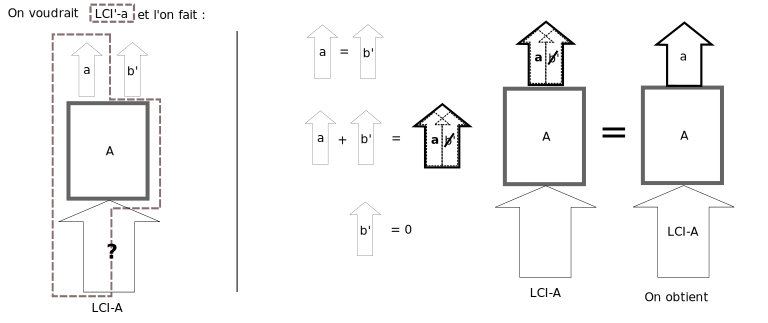
\includegraphics[width=\textwidth]{/home/rudy/Documents/rudy/01_These/11_production/01_COMMUNICATION/figures/allocation/LS_allocation.pdf}
\caption{Représentation de la méthode LSA.}
\label{fig:Lump-Sum}
\end{figure}

\figbox{Les flux relatifs aux commodités secondaire $\forall(k,J)\in \mathcal{J}|k = j,i\in \bullet$ sont considérés comme nuls.
Toute la production ($g_{J}$) est considérée comme primaire ($\wp$)
\exbox{\blockcquote[traduction. LSA]{majeau-bettez_unified_2014}{
Un champ de produisant de 5 tonnes (t) de céréales et 2 t de paille, [\ldots], serait modélisé comme la production, uniquement, de 7 tonnes de céréales.
%A field producing 5 tonnes (t) of grain and 2 t of straw, for example, would be modeled as producing 7 t of grain as its single output.
}
La somme est toujours de 7, mais les céréales passe de 5 à 7 et la paille de 2 à 0.
}
}



La somme groupée (LSA) ne respecte pas le principe de conservation des productions~\cite{majeau-bettez_unified_2014}.
Notez que nous considérons une conservation avec catégorisation.
La masse totale reste la somme de celles des coproduits.
Mais les flux, des coproduits non retenu, autant que du \textit{principal}, sont perturbés.
%Il nous parait peu légitime de développer plus encore des modes de décision ne respectant pas les lois connues de la physiques.
%Cela serait en tout cas poursuivre le développement des critiques à l'encontre de la méthode.
%Nous développerons plus particulièrement la question de la conservation des différentes "balances".

\subsubsection{PSA~: Product Substitution Allocation}

%\colorbox{yellow}{??? PSA et AAA dans une seule sous-section ???}

\begin{equation}
 \label{eq:Majeau unified equation PSA}
 z_{iJj}=
 \begin{cases} a_{iJj}v_{jJ} = u_{iJ} - \displaystyle\sum_{k|(k,J)\in\mathcal{J}} \xi_{ik}v_{kJ} \quad \forall(j,J)\wp,i\in \bullet 
 \\
 0 \quad \forall(j,J)\in \mathcal{J}|k = j,i\in \bullet
 \end{cases}
\end{equation}

La représentation de l'équation~\ref{eq:Majeau unified equation PSA} donne la figure~\ref{fig:PSA-FR}.
\begin{figure}[htbp]
\resizebox{1.00\textwidth}{!}{
\input{/home/rudy/Documents/rudy/01_These/11_production/01_COMMUNICATION/figures/allocation/PSA_allocation_xi.pdf_tex}
}
\caption{Représentation de la méthode PSA, avec un pont de procédé multi-fonctionnel (B-C).}
\label{fig:PSA-FR}
\end{figure}
\figbox{
Lisons conjointement l'équation~\eqref{eq:Majeau unified equation PSA} et la figure~\ref{fig:PSA-FR}.
Sur la représentation graphique, un 'pont' de substitution est représenté.
Pour accéder au produit b au sein du procédé multifonctionnel B, le coproduit c' et crédité à B depuis l'activité C, mono-productrice de c.
Les coproduits sont annulés dans l'activité traitée ($0 \forall(j,J)\in \mathcal{J}|k = j,i\in \bullet$) et la production \textit{principale} ($\forall(j,J)\wp,i\in \bullet$) est `crédité' au taux de déplacement près ($\xi_{ik}$) des fonctions, commodités ($v_{kJ}$) jugées substituées. % ($ a_{iJj}v_{jJ} = u_{iJ} - \sum_{k|(k,J)\in\mathcal{J}} \xi_{ik}v_{kJ} \forall(j,J)\wp,i\in \bullet $). 
}

Les produits secondaires pourrait tout à fait être exprimés sous le terme $\xi_{ik}v_{kJ}$.
Ainsi non "annulés", une version 'PSA balanced' (en fonction évidement, car ni en masse ni en aucune autre unité) pourrait donc exister (à hypothèse de substituabilité valide).
Il ne resterait qu'à définir les relations d'équivalence ($\xi_{ik}$), signifiant la différence des produits substitué l'un à l'autre.
Ceci donnerait~:
\begin{equation}
 z_{iJj}=
 \begin{cases} a_{iJj}v_{jJ} = u_{iJ} - \displaystyle\sum_{k|(k,J)\in\mathcal{J}} \xi_{ik}v_{kJ} \quad \forall(j,J)\wp,i\in \bullet 
 \\
 \xi_{ik}v_{kJ} \quad \forall(j,J)\in \mathcal{J}|k = j,i\in \bullet
 \end{cases}
 \label{eq:PSA-Majeau_Balanced}
\end{equation}
En somme c'est une formulation très proche du modèle AAA que nous verrons immédiatement après, au coefficient d'équivalence près.
\subsubsection{AAA~: Alternate Activity Allocation}

\begin{equation}
 z_{iJj}= a_{iJj}v_{jJ} =
 \begin{cases} u_{iJ} - \displaystyle\sum_{k|(k,J)\in\mathcal{J}} a^{\Gamma}_{ik}v_{kJ} \quad \forall(j,J)\wp,i\in \bullet 
 \\
 a^{\Gamma}_{ik}v_{kJ} \quad \forall(j,J)\in \mathcal{J}|k = j,i\in \bullet
 \end{cases}
 \label{eq:Majeau unified equation AAA}
\end{equation}


\begin{figure}[htbp]
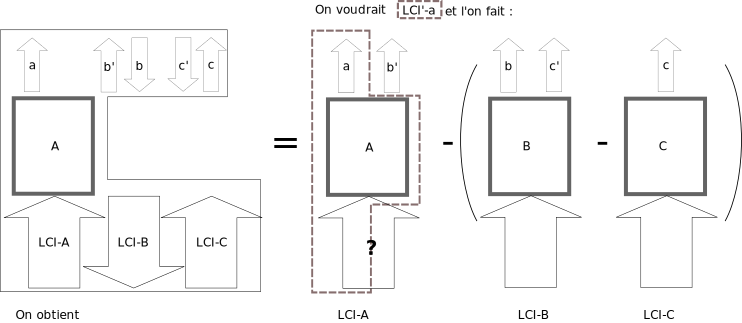
\includegraphics[width=\textwidth]{/home/rudy/Documents/rudy/01_These/11_production/01_COMMUNICATION/figures/allocation/AAA_allocation.pdf}
\caption{Représentation de la méthode AAA, avec un pont de procédé multi-fonctionnel (B-C).}
\label{fig:AAA-FR}
\end{figure}
\figbox{
L'équation \eqref{eq:Majeau unified equation AAA} est représentée dans la figure~\ref{fig:AAA-FR}.
La lecture est quasiment identique à Eq.\eqref{eq:Majeau unified equation PSA} et Fig.\ref{fig:PSA-FR} à ceci près que l'équivalence (du produit i au produit k) n'est pas donnée sur la base des produits avec $\xi_{ik}$ mais sur les procédés alternatifs par $a^{\Gamma}_{ik}$.

La nuance sensible dans entre l'expression (original) de PSA face à AAA est l'annulation des flux pour le domaine secondaire en PSA ($0 \forall(j,J)\in \mathcal{J}|k = j,i\in \bullet$).
}
%For example, one option is to ascribe to secondary coproducts the inputs that they would have required had they been produced as the primary product of some alternate activity (Figure 3:2.2) and ascribe the remainder of the joint requirements to the primary product.

%The total inputs and outputs of each activity remain identical to that recorded in the inventory (equation (8), decision variables ࢞U = ࢞V = 0). Thus, both primary and secondary productions remain available for intermediate or final use, that is, no observed flow is substituted, nothing is “avoided.”

AAA: "Alternate Activity Allocation" contient une contradiction dans sa présentation par \citeauthor{majeau-bettez_unified_2014}.
Les auteurs présentent cette méthode en indiquant qu'aucun flux observé n'est substitué et que rien n'est "évité" (référence à 'avoided burden').
%\footnote{
\blockcquote[traduction]{majeau-bettez_unified_2014}{
Le total des entrées et sorties de chaque activité reste identique à celui enregistré dans l'inventaire (équation (8) [de la publication d'origine], les variables de décision $ \Delta U = \Delta V = 0 $). Ainsi, les productions primaires et secondaires demeurent disponibles pour utilisation intermédiaire ou finale, i.e. \textbf{aucun flux observé n'est substitué, rien est "évité}."
%The total inputs and outputs of each activity remain identical to that recorded in the inventory (equation (8), decision variables $ \Delta U = \Delta V = 0$). Thus, both primary and secondary productions remain available for intermediate or final use, that is, no observed flow is substituted, nothing is “avoided.”
}
%}.
Or, ils décrivent également la méthode comme \blockcquote[traduction]{majeau-bettez_unified_2014}{
inscrivant aux produits secondaires, les flux qu'ils auraient requis s'ils avaient été produit en tant que production 'primaires' d'une activité alternative, laissant les autres flux nécessaires au produit primaire
}.
Les travaux cités en références sur cette méthode\footnote{
\blockcquote[traduction]{majeau-bettez_unified_2014}{
Des études telles que Cherubini et collègues (2011) et Weidema et Schmidt (2010) sont de bons exemples de cette modélisation
%Studies such as Cherubini and colleagues (2011) and Weidema and Schmidt (2010) are good examples of such modeling,
}},
traitent bien de commodités déplacées\footnote{
\blockcquote[traduction]{cherubini_influence_2011}{
le gaz naturel est supposé comme la source de chaleur et d'énergie déplacée
%natural gas is assumed as the source of the displaced heat and power
}.
\blockcquote[traduction]{weidema_avoiding_2010}{
Pour l'expansion du système, nous avons besoin du système supplémentaire de "bovins à viande», qui est \emph{déplacé} par la sortie supplémentaire de la viande de la vache laitière.}
Le système de la viande est exclusivement affecté la route des bovins de viande; c-a-d, dans le système étendu, aucune viande ne provient de vaches laitières.
%For system expansion, we need the additional system “meat cattle,” which is \emph{displaced} by the additional output of meat from the dairy cow.}
%The meat system is exclusively assigned the meat cattle route; that is, in the expanded system, no meat comes from the dairy cow.
}.
\textbf{Il s'agit donc bien de considérer une activité de \emph{substitution}.}
De même, une part des flux est évitée (soustraite) au produit 'principal' car présent au sein de l'alternative considérée.

%déjà critiqué par la communauté. \colorbox{red}{retrouver la ref}
L'AAA implique également d'après \citeauthor{majeau-bettez_unified_2014} certaines conditions nécessaires~:
%L'inventaire devrait être réparti entre différentes alternatives technologiques pour les co-productions \emph{secondaires}.
%Les conditions nécessaires au fonctionnement de ce système sont~:
\begin{itemize}
\item \blockcquote[traduction]{majeau-bettez_unified_2014}{la distinction robuste entre productions primaires et secondaires}
\item \blockcquote[traduction]{majeau-bettez_unified_2014}{la description d'une technologie alternative pour la production de chacun de ces co-produits "secondaires".}
\end{itemize}
Ce modèle fonctionne d'après les auteurs, même s'il n'y a pas de mono-production \textit{directement} pour chacun des co-produits immédiats grâce à un chaînage automatisé des ponts de substitution~\cite{majeau-bettez_unified_2014}.
Mais comment ce mécanisme d'allocation pourrait-il prendre fin sans procédé monofonctionnel pour chaque production à allouer "en bout de branche" (cf position du procédé C \ref{fig:AAA-FR})~?
Or, nous n'avons pas connaissance de procédé mono-flux.
Nous le développerons ultérieurement, la fonctionnalité est affaire de jugement et nous considérons des flux \emph{utiles} (jugement) comme fonctionnels.
Si nous complétons les éléments requis à la méthodologie AAA il faudra donc mentionner~: \emph{Jugement de substituabilité des produits entre-eux.}
%\colorbox{yellow}{brainstorming pour une annexe des flux non usuellement observés mais présent dans le but d'identifier un procédé mono-flux mono-fonctionnel ?}
%\begin{figure}[htbp]
%\includegraphics[width=\textwidth]{/home/rudy/Documents/rudy/01_These/11_production/01_COMMUNICATION/figures/allocation/Subsitution-fr.pdf}
%\caption{Représentation de la méthode PSA, avec pont de procédé multi-fonctionnel.}
%\label{fig:PSA-FR}
%\end{figure}
Le modèle nécessite l'existence systématique de procédés mono-fonctionnels, direct ou indirect, puisque chaque branche doit pouvoir s'arrêter.
L'absence de multifonctionnalité est théoriquement contournable car des cascades sont exploitables. 
\exbox{
Dans l'activité A produisant a,b et c~: A(ab'c'), a est `isolable' par B(bc'') ou B(b) + C(c) ou C(cb'') ou via P(pq'r'f') + T(tpb''') + V(vt') + Q(qs') \ldots
Les lecteurs comprendront aisément les limites pratiques à la possibilité théorique.
Car il est également crucialement requit que soient considérés substituables les différents produits modélisés (b' issu de l'activité A est considéré comme substituable à b de l'activité B etc.).
Ceci fait beaucoup de substitution à accorder.
D'où le commentaire de \citeauthor{heijungs_allocation_2007} d'un trop grand nombre d'hypothèses à gérer.
Et encore faut-il l'accepter même une seule fois.
}
Ainsi
$
%\begin{equation}
a \equiv ab' -(bc' -(cd' - d))\equiv a = ab -(bc -(cd - d))
%\end{equation}
$.
Et il en va de même pour les activités et leur impacts, comme précisé à l'introduction de cette section au \ref{subsec:Détails des méthodes}.

\subsubsection{PA~: Partitioning allocation, Allocation par partition}
L'allocation par partition est nécessaire pour l'évaluation comparative sur la base de l'\emph{unicité} de l'\gls{UF}, lorsque deux co-fonctions sont produites simultanément sans qu'il soit possible de les subdiviser en systèmes indépendants par les lois de la physique et dans une perspective de soutenabilité forte rejetant la substitution des produits ou des filières technologiques et leurs impacts.

Se pose la question~: Comment peuvent être allouées des parts de l'inventaire à chaque fonction résultante, chaque flux fonctionnel ?

Nous allons développer dans cette section ce mode de traitement de la multifonctionnalité.
Nous commençons ici par le présenter dans son état actuel.
%Allocation is needed when linked co-functions arise that cannot be subdivided into reduced systems by the laws of physics.

%How the allocate shares of the inventory to each resulting functions (functional flows)?
Certaines études cherchent la "meilleure" clef d'allocation (masse, énergie, devise), respectivement au champs d'application (carburant, nourriture, traitement des \emph{déchets} etc.)~\cite{silva_wood-based_2014, ayer_co-product_2006, cherubini_influence_2011}.
%Some studies search \emph{the best} allocation key (mass, energy, money) respectively to the application fields (fuels, food, waste treatment)~\cite{silva_wood-based_2014, ayer_co-product_2006, cherubini_influence_2011}.
%metal dubreuil ; 
%rejecting political ground Pelletier
%And this generate sector application specific rules.
\citeauthor{luo_allocation_2009} ont déclaré que \blockcquote{luo_allocation_2009}{mélanger les méthodes d'allocation dans un même cas d'étude n'est pas \emph{recommandable}}\footnote{
\citeauthor{luo_allocation_2009} dans cette étude traitent autant des méthodes que des clefs d'allocation au sein de la méthode par partition.
L'étude en question comprend d'ailleurs : la partition massique, économique et une expansion de système.
MA bio-CO2 exclu.
Economic Allocation
EA bio-CO2 exclu.
System Expansion.
La description de l'expansion sous-tend des coefficients de substitution de base physique.
L'\gls{UF} est composite mais unique.
\blockcquote{luo_allocation_2009}{
L'unité fonctionnelle utilisée dans les quatre solutions alternative est définie comme "un kilomètre de conduite automobile + valeur nutritive 13,6 kJ de maïs et de canne"\ldots
%The functional unit used in all four alternatives is defined as ‘one kilometre of car driving + nutritional value 13.6 kJ of corn and stover’\ldots
}
}, sans même justifier ce point de vu.
%\textsc{Luo} stated that \blockcquote{luo_allocation_2009}{mixing allocation methods in one case study is not advisable}.
Et de ce qui a été constaté, ce `mélange' n'est en effet pas réalisé (même application à tous le système).
Au mieux, différentes clefs sont testées en séquence en analyse de sensibilité ou pour un article à cette fin (comme ceux que nous discutons ici). % \colorbox{yellow}{!!!Reprendre les sources!!!}
%And from what we have observed, it is indeed not done.
%At best different allocation keys are sequentially observed.
Or, depuis le travail de \citeauthor{leontief_environmental_1970} il y a plus de \emph{quarante ans}, nous savons \emph{aujourd'hui} que l'ensemble de nos activités sont interconnectées~\cite{leontief_environmental_1970}. Donc, employer \textbf{une} \emph{règle sectorielle} pour calculer les allocations sur \emph{un système technico-social, \textbf{interconnectant} de fait \textbf{des secteurs différents}}, \emph{n'est pas adéquat}.
%But since the work of \textsc{Leontief}, we know all activities are connected~\cite{leontief_environmental_1970}.
%So using the rule of a particular sector and calling on a complete system seems inadequate.

Ce traitement monodimensionnel de l'allocation a été synthétisé par l'équipe \citeauthor*{majeau-bettez_unified_2014}.
Le principe énoncé est le suivant~:
~\blockcquote{majeau-bettez_unified_2014}{Toute allocation respectant la balance de production, qui répartisse les inventaires des nécessités sur les coproduits est représentée de manière générale par l'équation}
Eq.\eqref{eq:Majeau_unified_equation}

%\vspace{-.1cm}
\begin{equation}
 z_{iJj}=a_{iJj}v_{jJ} =
 \begin{cases} u_{iJ} - \displaystyle\sum_{k|(k,J)\in\mathcal{J}} \underline{a}_{iJk}v_{kJ} \quad \forall(j,J)\wp,i\in \bullet 
 \\
 \underline{a}_{iJk}v_{kJ} \quad \forall(k,J)\in \mathcal{J}|k = j,i\in \bullet
 \end{cases}
 \label{eq:Majeau_unified_equation}
\end{equation}
Avec les coefficients techniques exprimés par Eq.~\eqref{eq:technical_requirement_coefficient_majeau}
%with the technical coefficient expressed by: % \eref{eq:technical_requirement_coefficient_majeau}:
\begin{equation}
\underline{a}_{iJk}=u_{iJ}\frac{\psi_{kJ}}{\displaystyle\sum_{j\in\bullet}\psi_{jJ}v_{jJ}} \forall k|(k,J) \in \mathcal{J},i \in \bullet,J \in \ast
\label{eq:technical_requirement_coefficient_majeau}
\end{equation}
\figbox{
Aux flux utilisés (U) \emph{i} dans l'activité \emph{J} pour produire (V), de façon principale ($\wp$) la commodité \emph{j}, sont retirés des parts affectés aux coproductions secondaires ($\forall(k,J)\in \mathcal{J}|k = j,i\in \bullet$) sur la base de leur part suivant la clef d'allocation $\psi_{jJ}$, i.e. la part (fraction) $\frac{\psi_{kJ}}{\displaystyle\sum_{j\in\bullet}\psi_{jJ}v_{jJ}}$.

Pour rappel, 
\begin{description}
\item Les composants $z_{iJj}$ représentent les flux intermédiaires,
\item Les lettres capitales et $\ast$ représentent les activités.
\item Les lettres minuscules et les $\bullet$ signifient les nécessités (commodités).
\item $v_{kJ}$ composent la matrice de production.
\item $u_{iJ}$ composent la matrice des utilisations, consommations (untraceable, sans traçabilité).
\item ${a}_{iJk}$ sont les coefficients techniques.
\item $\mathcal{J}$ est le domaine des produits et activités \emph{secondaires}.
\item $\wp$ est le domaine des produits et activités \emph{primaires}.
\end{description}
}
%with $z_{iJj}$ the modelled intermediate flows, upper-case letters representing activities ; lower-case letters and $\bullet$ stand for commodities.
%$v_{kJ}$ is the supply matrix (productions).
%$u_{iJ}$ is the use matrix (untraceable).
%${a}_{iJk}$ are the technical coefficients (technical requirements).
%$\mathcal{J}$  is the domain of secondary products and activities.
%$\wp$ is the domain of primary products and activities.
\exbox{Prenons un exemple simple~:\\
%\newline
Dans l'activité \textbf{A}, à partir de~:
\begin{itemize}[noitemsep]
\item la consommation de 3~l de \textbf{s},
\item la consommation 1~kWh d'électricité \textbf{f}
\item l'émission de 10~g de \textbf{x} dans l'air
\item etc,
\end{itemize}
sont conjointement produits~:
\begin{itemize}
\item 100 unités de \textbf{a} pour une masse de 2~kg  (0.020~kg/unité) et un prix de 10~k€
\item 20 unités de \textbf{b'} pour un total de 1~kg (0.05~kg/unité) pour 2~k€.
\end{itemize} 

L'inventaire de l'activité A (les 3~l de \textbf{s}, le kWh d'électricité \textbf{f}, l'émission de 10~g de \textbf{x} dans l'air etc) est réparti~:
\begin{itemize}[noitemsep]
\item à 2/3 pour \textbf{a} et 1/3 pour \textbf{b'} suivant une clef massique.
\item à 5/6 pour \textbf{a} et 1/6 pour \textbf{b'} suivant une clef monétaire.
\end{itemize} 
Voyons comment, \emph{en suivant le formalisme présenté}\footnote{Ce qui brisera l'aspect de complexité de la formulation.}.\\
Soit \textbf{a}, arbitrairement le produit principal.
Prenons le cas de la clef massique.
Les 2/3 sont constitués sur la base du total (1), moins la part du secondaire (1/3), tel que présenté dans le développement suivant.\\
Le flux d'électricité \textbf{f}, alloué à la production de \textbf{a} dans l'activité A, c'est à dire $z_{fAa}$ est tel que\footnote{Le développement est présenté avec l'information dimensionnelle. N signifie Nombre d'Unité Produite.
Bien que sans dimension nous pensons que ces 'quantité d'item' aiderons la lecture.}~:\\
$z_{fAa} = u_{fA} - u_{fA} \times ( \frac{\mathit{masse_{b'A}/N_{b'A}}}{\mathit{masse_{b'A}/N_{b'A}}\times\mathit{N}_{b'A} + \mathit{masse_{aA}/N_{aA}}\times\mathit{N}_{aA}}) \times \mathit{N}_{b'A}\\
z_{fAa} = 1(kWh) - 1(kWh)(\frac{0.05(kg/N)}{0.05(kg/N)\times20(N_{b'A}) + 0.02(kg/N)\times100 (N_{aA})}) \times 20 (N_{b'A})\\
z_{fAa} = 1-1(\frac{1}{3})= 2/3 (kWh)$
}
Où se trouve le jugement de préférence dans cette équation générale \eqref{eq:Majeau_unified_equation}~?
Sous le PA, en dehors de la présence d'\emph{une} clef d'allocation, qui de fait est celle implicitement jugée comme \emph{absolument} plus importante que tout autre, il n'y en a pas de trace\footnote{Concernant PSA, AAA, LSA}.
%Where lies the preference judgement within the original equation that was stated in LCA theoretical framework?
%%Are preferences stated here?
%Apart from the fact that the allocation key used is the implicit \emph{single} important parameter, preferences are not stated here. %there is nothing more.
%\vspace{-0.3cm}
\subsubsection{Éviter l'allocation : expansion}
Nous commençons par présenter des avis divergents sur cette \textit{expansion}.
Puis nous exposons la pratique et la pensée derrière le terme.
Enfin nous présentons que l’expansion pourrait être.

\citeauthor{weidema_avoiding_2000} a avancé~\cite{weidema_avoiding_2000}, puis maintenu~\cite{weidema_avoiding_2010} que cela était \emph{toujours} réalisable.
%Mais c'est autre chose que l'expansion qui est défendu.
% \footnote{
\blockcquote[traduction]{weidema_avoiding_2000}{
Dans cet article, je conclus que l'allocation peut (et doit) \textbf{toujours} être évitée en ACV prospective. En ACV rétrospective, il est impossible d'exprimer un impératif concernant quelle procédure d'allocation appliquer, mais éviter l'allocation peut \textbf{toujours} être une option.
%In this article, I conclude that allocation can (and shall) always be avoided in prospective LCAs. In retrospective LCAs, it is not possible to express an imperative regarding what allocation procedure to apply, but avoiding allocation may still be an option.
}
%D'autres considèrent que l'expansion repose sur trop d'hypothèses et devrait être laissée hors d'un outil scientifique.
%\footnote{

Or, ceci n'est par exemple pas possible lors d'un examen comparatif entre deux co-production de même fonction (l'isolation de b' et b'' en traitement par substitution de b' et b''), car cela rejetterait l'hypothèse fondamentale de la méthode ($b' \equiv b''$)~\cite{kim_allocation_2002}.
%retrouver la ref sur system expansion SUBSTITUTION 
%\footnote{
%\exbox{
\blockcquote[traduction]{kim_allocation_2002}{
Cependant, cette approche [expansion - substitution] ne fonctionnerait pas pour une étude d'ACV dans lequel le but est de comparer les charges environnementales entre les différentes technologies de production d'éthanol.
%Une approche par l'expansion possible du système, qui pourrait atteindre l'objectif d'une telle étude ACV, serait de répartir les charges environnementales soit la farine de soja ou de l'huile de soja dans le système de broyage du soja en fonction des propriétés physiques ou des valeurs économiques, même si les procédures d'allocation ne seraient pas éliminées.
%However, \textbf{this approach would not work for an LCA study in which the goal of a study is to compare the environmental burdens between different ethanol production technologies}. A possible system expansion approach, that could meet the goal of such an LCA study, would be to allocate the environmental burdens to either soybean meal or soybean oil in the soybean milling system based on physical properties or economic values even though the allocation procedures would not be phased out."
}
%\citeauthor{kim_allocation_2002} expliquaient en effet que~:\blockcquote[traduction]{kim_allocation_2002}{
%L'hypothèse sous-jacente à l'approche de l'expansion du système est que les systèmes de produits avec une fonction équivalente ont les mêmes charges environnementales [9]. Par conséquent, les charges environnementales associées à l'éthanol à partir du broyage à sec sont supposés être équivalentes à celles qui sont associés à de l'éthanol à partir de broyage humide.
%%The underlying assumption in the system expansion approach is that product systems with an equivalent function have the same environmental burdens [9]. Hence, the environmental burdens associated with ethanol from dry milling are assumed to be equivalent to those associated with ethanol from wet milling.
%}
La littérature ne propose alors pas d'autre alternative que la proposition actuelle de partition.

\blockcquote[traduction]{cherubini_influence_2011}{
[\ldots] Tandis que Heijungs et Guinée analysent la logique et les problèmes, à la fois l'expansion et du partitionnement, ils concluent que la méthode d'expansion du système est généralement basée sur un trop grand nombre d'hypothèses, qui "doivent de préférence être laissées à l'extérieur d'un outil principalement scientifique" (Heijungs et en Guinée, 2007)~\cite{heijungs_allocation_2007}\footnote{\blockcquote[traduction]{heijungs_allocation_2007}{
Il apparaît que pour approcher les charges évitées, le nombre de "et si~?" hypothèses est si grand que les ACV sur le même sujet conduisent à des résultats assez divergents.
Puisque les questionnement "et si~?" ne peuvent pas recevoir de réponse non ambiguë, ces questions devraient de préférence être laissés à l'extérieur d'un outil principalement scientifique.
%It appears that for the avoided burdens approach, the number of ‘what-if’ assumptions is so large that LCAs on the same topic lead to quite diverging results.
%Since ‘what-if’ questions cannot be answered in an unambiguous way, such questions should preferably be left outside of a primarily scientific tool.
}.
%while Heijungs and Guinée analyze the logic and problems of both partitioning and system expansion, concluding that the system expansion method is usually based on a too large number of assumptions, which “should preferably be left outside of a primarily scientific tool” (Heijungs and Guinée, 2007).
}}.

{
%L'argumentation du début des années 2000 était la suivante.
%\blockcquote{weidema_avoiding_2000}{
%Because a system expansion may involve processes that also have multiple products, it has been suggested that there are situations in which system expansion
%would be impossible because it would involve an unending regression.
%}
%What is the counter argument on this point.
%> use "the market-based method of Weidema and colleagues (1999)"
%>> then it is an economic study
%
%information is lost in economical agregation
%
%there is no remaining information to build another judgment.
%
%> expansion = economic allocation + product and impact substituability
%{
%%FAIRE UNE TABLE AVEC ARGUMENTAIRE // CONTRE ARGUMENTAIRE WEIDEMA pour aider à la reformulation
%%
%%Trouver une autre forme de tableau (2 cases dessus, une case dessous)
%%thèse anti-thèse synthèse
%%|arg|contre-arg|
%%
%%|commentaire|
%
%%\begin{landscape}
%%\begin{longtabu} to \textwidth{some columns}
%%\caption[my caption]{my caption}
%%table code here
%%\end{longtabu}
%%\end{landscape}
%
%%\begin{landscape}
%%%\begin{longtabu} to \textwidth{some columns}
%%%\caption[my caption]{my caption}
%%%table code here
%%%\end{longtabu}
%%
%%\begin{longtable}{| p{7cm} | p{7cm} | p{5cm}|}
%%The following four obstacles to system expansion can be seen as part of the reason why thisoption has not generally been applied as a way toavoid allocation: & 
%%In this article, I conclude that allocation can(and shall) always be avoided in prospectiveLCAs. In retrospective LCAs, it is not possibleto express an imperative regarding what allocation procedure to apply, but avoiding allocationmay still be an option. I reach this conclusion byshowing how to overcome the four obstacleslisted above: & 
%%Commentaire\\ 
%%\hline
%%The following four obstacles to system expansion can be seen as part of the reason why this option has not generally been applied as a way to avoid allocation:  &
%%... I reach this conclusion by showing how to overcome the four obstacles listed above:  &
%%Commentaire\\ 
%%\hline 
%%1. In retrospective LCAs, there is typically no possibility for system expansion.
%%Retrospective studies typically seek to describe a status quo situation, in which there are no changes in production volume.
%%This obviously excludes the possibility of system expansion, because an expansion involves balancing a change in output volume of a co-product in one system with an equivalent change in the other systems to be compared, in order to maintain comparable product outputs from the systems.
%%The distinction between retrospective and prospective studies and its important consequences for the methodology (including the handling of co-products) has only recently been clarified (Tillman 1998; Weidema 1998).
%%It is still common to see retrospective studies applied for prospective purposes and a mix of methodologies and justifications without clear reference to the retrospective or prospective nature of the study.  &
%%1. By distinguishing clearly between retrospective and prospective studies (see next section)
%%, it is possible to distinguish between the situations in which system expansion is both possible and mandatory (prospective studies) and the situations in which system expansion is irrelevant or at least optional (retrospective studies).  &
%%Les études qualifiées de "retrospective" au sens attributionnelle ont tout autant que les études conséquentielles "prospective" un horizon temporelle incluant le futur et le passé.
%%Elles portent donc toutes des considérations sur les évolutions des productions et des marchés (output volumes).
%%L'hypothèse de volumes constants (que l'on retrouve en hypothèse pour l'inversion de Leontief) serait problématique pour tant pour l'antériorité (horizon temporel passé) que pour le futur.
%%Le premier argument 'contre' une expansion qui modifierait les volumes de production et donc valide, non pas pour les prospective ou retrospective mais pour toute partie historique des deux types d'études.
%%\\ 
%%2. It has been regarded as too difficult, too uncertain, or even impossible to identify which processes are affected when balancing a change in demand for (or supply of) a specific co-product.  &
%%2. By applying the market-based method of Weidema and colleagues (1999), I show that it is always possible, and seldom difficult, to identify the processes affected by a change in demand.
%%The uncertainty of this determination and the fundamental uncertainty of future market situations are inherent to the method, but can be neither a theoretical nor a practical argument against system expansion. &
%%La substitution par critère économique des produits maintien l'expansion substitution dans l'hypothèse de soutenabilité faible (qu'il s'agisse de la variante AAA ou PSA).
%%Plus qu'une question de difficulté, c'est une question de jugement sur la substituabilité pour la soutenabilité qui s'oppose à ce principe.\\ 
%%3. Because a system expansion may involve processes that also have multiple products, it has been suggested that there are situations in which system expansion would be impossible because it would involve an unending regression.  &
%%3. The problem of unending regression is eliminated by applying the method mentioned above, which provides clear cut-off criteria (a process is either included or excluded from the studied system) and reduces the number of processes that may possibly be involved in a system expansion (for details, see the section called: “Displaced Processes that Have Multiple Products”).
%%(ladite section)> When a displaced process yields not only the displaced product, but also other co-products, these co-products are also displaced and the demand for them must now be met in another way.
%%Thus, the procedure must be repeated for these co-products, but with a negative sign.
%%If this leads again to another process with multiple products, one might fear that this system expansion would continue without end.
%%The number of possible processes involved in the system expansion, however, is limited by the very procedure, because:
%%• the number of markets affected by each displaced process is limited, and the displaced process is only that specific supplier to each market, which is most sensitive to a change in demand,
%%• the four rules for system expansion provide clear cut-offs between the different product systems involved (a process is either included or excluded from the studied system),
%%• for each time the system expansion is iterated, both the economic value and the volume of the displaced processes tend to decrease, because in each iteration the avoided product is the determining coproduct of the displaced process and therefore typically of higher value (and often also larger in quantity) than the dependent coproducts, which go on to the next iteration. &
%%Double emploi du contre-argument 2 : Substituabilité sur la base de critère économique.
%%Question de suite géométrique de raison inférieure à un pour la convergence.\footnote{Raison inférieur à un sur l'hypothèse que le produit de susbstitution (co-produit) est de moindre qualité que le produit de même fonction déplacé. Cette commodité déplacée, "primaire", est (hypothèse) également produit en plus grande quantité.}
%%La fraction déplacé tend vers zéro.
%%C'est la base du raisonnement économique.
%%Il est donc mathématiquement juste.
%%Mais les mathématiques sont pour les modèles et comporte des hypothèses.
%%Il y a, non pas substituabilité entre un petit nombre de produits mais bien sur l'ensemble des "marchés".
%%Une commodité hors de la sphère monétaire mets par exemple quelques grains de sable dans ce "modèle".
%% \\ 
%%4. When a by-product does not substitute for another product, system expansion may be regarded as incompatible with the requirement that compared systems must have identical functions.  &
%%4. It is shown that by-products practically always substitute for other products, and even when this may not be the case, the studied systems are still comparable. &
%%"by-products practically always substitute for other products" On what basis, {{citation needed}}, authority etc.
%%"the studied systems are still comparable."
%%> Confrontation de paniers de fonctions différentes à évaluer tout de même (plus tard).
%%La multifonctionnalité n'a pas été résolue elle est repoussé.
%% \\ 
%%\hline
%%\caption{Argumentaire de Bo Weidema sur l'expansion en 2000}
%%\label{tab:expansion_weidema_arguments}
%%\end{longtable}
%%\end{landscape}
%}
}
Or, grattons un peu la surface et voyons les mécanismes et arguments employés par ses défenseurs.

\citeauthor{weidema_avoiding_2010} posent l'expansion comme conservatrice des balances et la partition (allocation) comme systématique perturbatrice.
%\footnote{
\blockcquote[traduction]{weidema_avoiding_2010}{
Ici, il est intéressant de noter que \textbf{l'expansion du système assure toujours des bilans de masse et de l'énergie, alors que l'allocation échoue presque toujours ce test}.
En bref, l'allocation brise le système original en deux systèmes artificiels ou plus selon une clé de répartition, et le seul équilibre qui reste intact dans les systèmes résultant est celui donné par la clé de répartition.
%Here, it is interesting to note that \textbf{system expansion always ensures mass and energy balances, whereas allocation nearly always fails this test}.
%In brief, allocation breaks up the original system into two or more artificial systems according to an allocation key, and the only balance that remains intact in the resulting systems is that given by the allocation key.
%With mass allocation, the mass balance remains intact, but energy and elemental balances are skewed; with economic allocation, none of the physical balances remains intact except if by chance a physical parameter follows the price of the products.
[\dots]
Avec l'expansion du système, les processus unitaires affectés sont agrandis ou réduits, mais il n'y a pas de partition artificielle, et parce que les systèmes qui en résultent sont de simples sommes des procédés unitaires concernés, dont chacune \textbf{maintient ses équilibres physiques intacts}, les systèmes résultant ont aussi tous leurs équilibres physiques intacts.
%With system expansion, the affected unit processes are scaled up or down, but there is no artificial partitioning, and because the resulting systems are simple sums of the affected unit processes, each of which \textbf{maintains its physical balances intact}, the resulting systems also have all physical balances intact.
}
%}.

Nuançons dès maintenant l'affirmation de \citeauthor{weidema_avoiding_2010} sur la conservation en extension.
"unit processes are scaled up or down", lorsque les procédés employés sont "mis à l'échelle", les volumes de leurs productions et consommations sont modifiés.
Donc les procédés appellent ou émettent des quantités, soit plus faibles, soit plus grande dans le système de production générale.
Celui-ci s'en trouve donc perturbé.
%\colorbox{yellow}{SCHEMA + FORMULE pour appuyer ce très juste propos}

Les propos de \citeauthor{weidema_avoiding_2010} pourraient paraître d'autant plus curieux face à la classification de \citeauthor{majeau-bettez_unified_2014} (Two General Allocation Strategies) où seuls PA et AAA conservent les bilans de produits~\cite{majeau-bettez_unified_2014}.
%D'autant plus que selon cet article, l'approche par \emph{partition} conserve les balances.

Lors de ces affirmations il est question \emph{des} balance\emph{s} globale et locales, balance du système et balances des procédés.
C'est a dire que pour \citeauthor{majeau-bettez_unified_2014} 
%\colorbox{yellow}{(autres publi sur la conservation)}
l'ensemble des produits initialement non alloués est conservé sur l'ensemble des allocations.
\textbf{La somme des parties reste égale au tout.}
\citeauthor{weidema_avoiding_2010} indiquent eux que pris en isolation, le "modèle de système unitaire monofonctionnel", \emph{lui} n'est plus équilibré.
Nos théoriciens semblent s'opposer, mais ils ne traitent pas des même équilibres.
%Ce modèle n'a bien sûr pas d'existence autre que théorique.

Voyons d'autres arguments.
\blockcquote[traduction]{weidema_avoiding_2010}{
En appliquant la méthode de Weidema et collègues (1999) \textbf{basée sur le marché}, je montre qu'il est toujours possible, et rarement difficile, d'identifier les processus affectés par un changement dans la demande [identifier le substitut]. L'incertitude de cette détermination et de l'incertitude fondamentale des futures situations de marché sont inhérentes à la méthode, mais ne peut être un argument ni théorique ni pratique contre l'expansion du système.}
%By applying the market-based method of Weidema and colleagues (1999), I show that it is always possible, and seldom difficult, to identify the processes affected by a change in demand. The uncertainty of this determination and the fundamental uncertainty of future market situations are inherent to the method, but can be neither a theoretical nor a practical argument against system expansion.}
\blockcquote[traduction]{weidema_avoiding_2010}{
%Tout d'abord,
[\ldots] l'allocation implique généralement une partition plus ou moins arbitraire du processus de co-production sur ses co-produits, sans tenir compte de la mesure dans laquelle un changement dans la quantité de ces co-produits affecte réellement la sortie fonctionnelle et d'autres échanges de la co-production processus.
%Deuxièmement, l'allocation ne tient pas compte des effets qu'un co-produit peut avoir sur le sort ultérieur des autres coproduits, qui est, les effets de déplacement et un traitement supplémentaire des co-produits avant le déplacement a lieu.
%First, allocation typically involves a more or less arbitrary partitioning of the co-producing process over its co-products, without consideration of the extent to which a change in the amount of these co-products actually affects the functional output and other exchanges of the co-producing process. Second, allocation ignores the effects that a co-product may have on the further fate of the other coproducts, that is, displacement effects and additional treatment of the co-products before displacement takes place.
}
Cela apparaît clairement, ce qui est désigné par l'expansion est en fait de la substitution sur la base majoritaire d'une allocation économique (via le marché).

Vous l'aurez compris, l'antagonisme a pour centre la subjectivité.
Des thèses différentes s'opposent sans que ne soit attaqué leur fondement commun.\\
A: Tout est toujours substituable sous critère économique.\\
Donc il est mathématiquement toujours possible d'appliquer l'expansion-substitution.\\
B: La substituabilité elle-même est une hypothèse problématique. Partitionner requière l'emploi de critères subjectifs.\\
A':Ce modèle (partition) repose sur le choix \href{http://www.cnrtl.fr/definition/arbitraire}{arbitraire} de la clef d'allocation.\\
B':Les hypothèses de substituabilité ne sont pas gérables\ldots\\
Ce qui n'est pas remis en cause est qui sous-tend les deux parties est qu'il y ait à trouver une unique et réelle description monofonctionnelle du système.


Ce qui est décrit comme problématique par \citeauthor{weidema_avoiding_2010} est en fait une incompréhension entre un objectif d'allocation pour produire une \emph{observation} ou celle avançant déjà dans l'\emph{évaluation}.
Il ne s'agit de modéliser des procédés unitaires monofonctionnels.
Ceux-ci n'existent pas.
C'est ce que frôlent du doigt \citeauthor{cruze_allocation_2014}.
Selon eux toutes les formes d'allocation sont juste.
Elles ne font qu'éclairer le problème de manière incomplète sous l'angle sélectionner pour l'attribution d'une part de l'inventaire.
\blockcquote[traduction]{cruze_allocation_2014}{
L'allocation par partition n'explore seulement qu'un petit sous-ensemble de solutions à un problème qui est mal posé en ce sens qu'il n'a pas une seule solution, mais potentiellement une infinité de solutions.
%partitioning explores only a small subset of solutions to a problem that is ill-posed in the sense that (1) it does not have just one solution, but potentially infinitely many solutions
}
Mais ces auteurs rejettent la piste de la subjectivité pour retomber dans le dogme de la donnée et du technocratisme.
\blockcquote[traduction de la conclusion]{cruze_allocation_2014}{
Plutôt que de compter sur une partition, une meilleure approche serait de rechercher des données supplémentaires ou un jugement d'expert afin que au moins le paramètre d'intérêt (l'inventaire monofonctionnel) devienne estimable.
%Rather than relying on partitioning, a better approach
%would be to seek out additional data or expert judgment so that
%at least the parameter (single product inventory) of interest
%becomes estimable.
}

Nous n'avons pas à les modéliser.
Construire l'inventaire, c'est déjà évaluer.
Mais pour accepter cela, il faut intégrer la subjectivité intrinsèque de la démarche d'évaluation.
Nous noterons à nouveau qu'une approche par expansion (ici sans substitution ni mise à l'échelle) permettrait de retarder l'usage du jugement mais pas de sans passer.


\keybox{
\textbf{"Avoiding allocation"}, les procédés sont multifonctionnels, prenons les comme tels.
Mais cette position revient à devoir observer et évaluer des alternatives sur des bases fonctionnelles différentes.
Pour conserver ces fonctions, le principe devrait reposer sur l'extension du système étudié.
Ceci implique de confronter non plus les alternatives sur la seule base de l'unité fonctionnelle, mais sur l'ensemble des fonctionnalités résultantes.
Traiter le jugement de valeur en fin de méthode n'est en rien une méthode de traitement.
C'est un ordonnancement de tâches, pas leurs réalisations.
}
Et parce que les praticiens comme les théoriciens ont jusqu'ici jugé nécessaire de conserver l'\emph{unicité} de l'unité fonctionnelle, c'est une approche par substituabilité qui suit généralement (cf les deux sous-section précédentes).


Hors amalgame de désignation Expansion - Substitution, observons un dernier point.
Pour traiter d'un procédé A donnant a et b', l'analyse est étendue.
Mais dans l'amont et l'aval des activités liées à a comme b' se trouvent d, e, f etc.
S'en suivra donc l'évaluation d'un quantum de a à une autre fraction de a' mais plus exactement a(+ d, e, f, etc.) face à a'(+ m,n,o,p etc.).
\keybox{
Ces ensembles de fonctions (comme l'ont justement souligné \citeauthor{weidema_avoiding_2010}) naîtront à des temporalité différentes, tout comme leurs impacts.
Pour tenir compte des horizons temporels choisis,
%(cf section \ref{label})
comme des phénomènes de concentration pour les impacts
%(cf section \ref{label})
,
il faudra probablement en terme d'ordonnancement commencer par l'expansion avant de réaliser le traitement de la multifonctionnalité.
La question sera donc finalement de traiter une évaluation comparative sur la base d'une unité fonctionnelle unique ou de réaliser un choix parmi des alternatives conduisant à la confrontation de groupes de fonctions de quantités et de natures variables.
}

%\subsubsection{Partitionner}

\subsection{Reclassification, conclusion partielle}
\keybox{
Il ne reste donc plus que \emph{PA: "Partitioning Allocation"}.
C'est le seul choix logique (consistant) sous une perspective de soutenabilité forte (excluant la substitution) en dehors d'un traitement global après expansion sans mise à l'échelle (conservation des balances des systèmes unitaire, comme du système global) .
}
La PA peut être rendue consistante par l'emploi de méthodes de décision multi-critère via l'adjonction que nous proposons.
Nous allons développer le traitement par partition en section~\ref{sec:partitionning}

Ceci donne la classification de la figure~\ref{fig:MULTIFONCTIONNATLITE_REclassification}.
\begin{figure}[htbp]
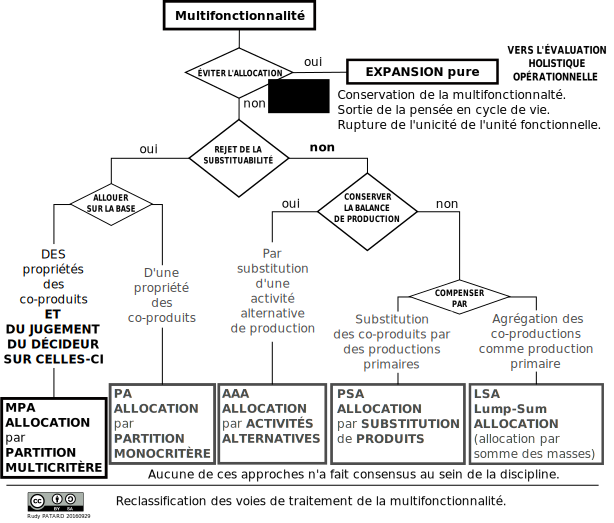
\includegraphics[width=\textwidth]{/home/rudy/Documents/rudy/01_These/11_production/01_COMMUNICATION/figures/allocation/Traitement_de_la_multifonctionnalite_reclassification.pdf}
\caption{Re-classification des approches de résolutions de la multifonctionnalité.}
\label{fig:MULTIFONCTIONNATLITE_REclassification}
\end{figure}
\figbox{
En somme sous le paradigme de l'ACV avec unicité de l'\gls{UF} nous avons deux approches, la partition et la substitution, sous ses diverses variantes, conservatrices ou non de balances de production, LSA, PSA, AAA.
%Dans l'approche par partition l'expansion peut être incluse comme première étape (ordonnancement).
L'ajout de fonctions au modèle nécessite la comparaison d'alternatives répondant à diverses fonctions.
Sous le principe de l’expansion pure, la préférence entre les alternatives socio-techniques est définie entre deux ensembles (fonctions et impacts) de dimensions et quantifications différentes.
L'approche par partition pose le jugement entre fonctions à l'échelle du procédé de premier plan.
Il s'agit du niveau duquel est délivré le flux fonctionnel de référence.
La partition alloue l'inventaire entre les flux fonctionnels issus de l'activité traitée.
Cette méthode permet le traitement de chacune des alternatives socio-techniques observées sans qu'un cas d'étude ne soit non solvable par cette méthode\footnote{Contrairement à l'opposition de produits de substitution, b et b', comme vu plus haut.}.
}

\section{Allocation par partition revisitée}
\label{sec:partitionning}
Nous allons dans cette partie apporter des modifications à l'équation générale de \citeauthor{majeau-bettez_unified_2014}.
Nous présentons tout d'abord l'ajout explicite des préférences.
Après une présentation du modèle nous suivrons sont comportements suivant les domaines parcourus par les propriétés des flux.
Ceci nous amènera à redéfinir le statut du déchets.
Nous dépasserons le statut de déchet économique pour obtenir le déchets économique \textbf{et} \emph{d'usage}.
Ceci nous conduira à réévaluer les frontières des systèmes en responsabilités et en appréciations pour finalement juger de l'importance de l'intention (volonté de création du flux) et de sa destination (son usage effectif).

\subsection{Un modèle d'allocation avec préférences explicites}
Dans la formulation précédente de l'allocation par partition, chaque procédé a \emph{une} et une seule propriété intensive déclarée comme clef d'allocation ($\psi_{iJ}$).
Développer la gamme de propriétés considérées donne un indice additionnel~: $\psi_{niJ}$.
%In the previous formulation each process has \emph{one} intensive property declared as allocation key ($\psi_{iJ}$).
%Developing the range of properties to consider we get an additional indices: $\psi_{niJ}$.
%\footnote{
$n$ sont les indices pour les propriétés des flux fonctionnels produits considérés et $\mathcal{N}$ est le domaine des propriétés, ainsi $n \in \mathcal{N}$.
$N$ est la fraction de $\mathcal{N}$ \emph{concernée par tous les flux des activités} $J$ \emph{étudiés pour l'allocation}.
%$n$ is the indices for the properties of commodities we are considering
%and $\mathcal{N}$ is the domain of properties, so $n \in \mathcal{N}$.
%$N$ is the fraction of $\mathcal{N}$ \emph{concerned by all flows of the activity} $J$ \emph{studied for allocation}.
%}
\footnote{Ceci signifie que pour l'implémentation, le facteur d'importance relative devra être dérivé de chaque procédé appelé pour traitement de multifonctionnalité.}
Le système de préférence est joint au ratio de propriétés dans l'expression des coefficients techniques dans l'équation \eqref{eq:technical_coefficient_multicriteria}.
Le coefficient technique devient ainsi~:
%The preference system is joined to the property ratio in the expression of technical coefficients in the following equation: \eref{eq:technical_coefficient_multicriteria}.
%The technical coefficients thus become:

%\footnote{This means that for implementation, the relative importance factor shall be derived at each process calling for allocation.}
%The preference system is joined to the property ratio in the expression of technical coefficients in the following equation: \eref{eq:technical_coefficient_multicriteria}.
%The technical coefficients thus become:
% Giving as a result the expression of the ``technical requirement matrix'':

%\begin{center}
%\colorbox{yellow}{ Recherche de formulation sur le terme de préférence 
%$\frac{\mathit{Pref}(\psi_{njJ})}{\displaystyle\sum_{n \in N} \mathit{Pref}(\psi_{njJ})}$
%}
%
%ou
%
%\colorbox{yellow}{
%${\mathit{Pref}(\psi_{njJ} / N)}$, moins orienté sur une méthode de dérivation.
%}
%\end{center}

\begin{equation}
  \begin{split}
  & a_{iJk}=u_{iJ}\displaystyle\sum_{n \in N}\dfrac{\psi_{nkJ}}{\displaystyle\sum_{j\in\bullet}\psi_{njJ}v_{jJ}} \mathit{Pref}(\psi_{njJ/N})
  \\
%   &  \forall k|(k,J) \in \mathcal{J},i \in \bullet,J \in \ast, N \in \mathcal{N}
  \end{split}
  \label{eq:technical_coefficient_multicriteria}
\end{equation}
La conservation de la balance globale de production qui résulte de la normalisation aux propriétés présentes et aux préférences respectives est présentée Eq.~\eqref{eq:production_balance}\footnote{Il sera compris qu'ici les pseudo-procédés monofonctionnels non \emph{plus aucune} 'balance' de propriété d'équilibrée, conformément à la description de \citeauthor{weidema_avoiding_2010}.}.
%with the production balance conservation resulting from the normalization to present properties and respective preferences: % in \eref{eq:production_balance}.
%
%$
%1 = \sum_{n,k}\left\{\frac{\psi_{nkJ}v_{jJ}}{\sum_{j\in\bullet}\psi_{njJ}v_{jJ}} \frac{\mathit{Pref}(\psi_{njJ})}{\sum_{n \in N} \mathit{Pref}(\psi_{njJ})} \right\}
%$
%
\begin{equation}
1 = \displaystyle\sum_{n,k}\left\{\frac{\psi_{nkJ}v_{jJ}}{\displaystyle\sum_{j\in\bullet}\psi_{njJ}v_{jJ}} \mathit{Pref}(\psi_{njJ/N}) \right\}
\label{eq:production_balance}
\end{equation}
%
%Thus the distinction between primary, secondary product or elementary flows and product flows are dismissed.

Le formalisme de \citeauthor{majeau-bettez_unified_2014}
\blockcquote[traduction]{majeau-bettez_unified_2014}{
[\ldots] pourrait faire croire que cela limite [le] cadre de répartition des activités dans le cas d'un produit primaire clairement identifiable, mais ce n'est pas le cas.
À ce niveau de généralité, cela signifie simplement que notre description de l'allocation est exprimée en termes d'un produit choisi parmi ses coproduits.
Pour de nombreuses techniques d'allocation, cette sélection peut être complètement arbitraire.
%This nomenclature might make it seem as though this limits our framework to allocation of activities with a clearly identifiable primary product, but it is not the case. At this level of generality, it merely means that our description of allocation is expressed in terms of one product selected among its coproducts. For many allocation techniques, this selection can be completely arbitrary.
}
La distinction entre \emph{primaire} et \emph{secondaire} n'est maintenant plus nécessaire, qu'elle fut arbitraire ou d'une subjectivité collective\footnote{Ce qui pourrait être considéré principal serait le flux recueillant le plus de préférence.}.
Nous pouvons donc passé d'une distinction `arbitraire mais sans conséquence' (apparente), à `évité'.
%The identification of \emph{primary} production is no longer \emph{arbitrary}\footnote{It is the most valued flow according to the decision maker preferences}.
%So we can go from consequence free
%\footnote{
%\blockcquote{majeau-bettez_unified_2014}{This nomenclature might make it seem as though this limits our framework to allocation of activities with a clearly identifiable primary product, but it is not the case. At this level of generality, it merely means that our description of allocation is expressed in
%terms of one product selected among its coproducts. For many allocation techniques, this selection can be completely arbitrary.}
%},
%to avoided.
Éliminer la dualité primaire -- secondaire simplifie également le formalisme de ~\citeauthor{majeau-bettez_unified_2014} et les notations consécutives à la distinction entre primaire et secondaire ($\underline{a}_{iJk}$ ; $\tilde{\underline{A}}$\ldots).

%Clearing the duality primary -- secondary products simplifies \textsc{Majeau-Bettez}~'s work~\cite{majeau-bettez_unified_2014} and notations ($\underline{a}_{iJk}$ ; $\tilde{\underline{A}}$$\ldots$).
Les flux alloués deviennent~:
%The allocated flows become:
\begin{equation}
%\begin{align*}
 z_{iJj}=a_{iJj}v_{jJ}= u_{iJ}\sum_{n,k}\dfrac{\psi_{nkJ}v_{jJ}}{\displaystyle\sum_{j\in\bullet}\psi_{njJ}v_{jJ}}\mathit{Pref}(\psi_{njJ/N})\\
\forall k,i,j \in \bullet | \forall J \in \ast | \forall n \in \mathcal{N}
\label{eq:multicriteria_allocated_flows}
%\end{align*}
%%\begin{align*}
% z_{iJj}=a_{iJj}v_{jJ}= & u_{iJ}\sum_{n,k}\dfrac{\psi_{nkJ}v_{jJ}}{\displaystyle\sum_{j\in\bullet}\psi_{njJ}v_{jJ}}\mathit{Pref}(\psi_{njJ/N})\\
%&\forall k,i,j \in \bullet | \forall J \in \ast | \forall n \in \mathcal{N}
%\label{eq:multicriteria_allocated_flows}
%%\end{align*}
\end{equation}
\figbox{Nous précisons dans l'Eq.\eqref{eq:multicriteria_allocated_flows}, que l'expression du flux alloué vaut quelques soient les commodités, quelques soient les activités et quelques soient les propriétés.}
%

!!! PB avec l'exbox l 1016 à 1077

%\exbox{
%Reprenons notre exemple simple~:\\
%%\newline
%{\scriptsize
%(Rappel) Dans l'activité \textbf{A}, à partir de~:
%\begin{itemize}[noitemsep]
%\item la consommation de 3~l de \textbf{s},
%\item la consommation 1~kWh d'électricité \textbf{f}
%\item l'émission de 10~g de \textbf{x} dans l'air
%\item etc,
%\end{itemize}
%sont conjointement produits~:
%\begin{itemize}
%\item 100 unités de \textbf{a} pour une masse de 2~kg  (0.020~kg/unité) et un prix de 10~k€ (100~€/unité),
%\item 20 unités de \textbf{b'} pour un total de 1~kg (0.05~kg/unité) pour 2~k€ (100~€/unité).
%\end{itemize} 
%
%L'inventaire de l'activité A (les 3~l de \textbf{s}, le kWh d'électricité \textbf{f}, l'émission de 10~g de \textbf{x} dans l'air etc) était réparti~:
%\begin{itemize}[noitemsep]
%\item à 2/3 pour \textbf{a} et 1/3 pour \textbf{b'} suivant une clef massique.
%\item à 5/6 pour \textbf{a} et 1/6 pour \textbf{b'} suivant une clef monétaire.
%\end{itemize} 
%}
%La préférence entre une valorisation monétaire et une valorisation massique est définie par le décideur fictif à~:
%\begin{center}
%$
%\begin{matrix}
%	& masse & prix & Priorité \\
%masse & 1 & 1/4 & 0.2 \\
%prix & 4 & 1 & 0.8 \\
%\end{matrix}
%$
%\end{center}
%
%Voyons comment est maintenant produite l'allocation, \emph{en suivant le formalisme présenté}.
%Le flux d'électricité \textbf{f}, alloué à la production de \textbf{a} dans l'activité A, c'est à dire $z_{fAa}$ est tel que~:\\
%%\footnote{Le développement est présenté avec l'information dimensionnelle. N signifie Nombre d'Unité Produite.
%%Bien que sans dimension nous pensons que ces 'quantité d'item' aiderons la lecture.}
%%}
%
%{\small
%\begin{equation}
%\begin{align*}
%z_{fAa} = & u_{fA}(\\
%&\frac{\mathit{masse_{aA}/N_{aA}}}{(\mathit{masse_{b'A}/N_{b'A}}) \mathit{N}_{b'A} + (\mathit{masse_{aA}/N_{aA}})\mathit{N}_{aA}} \mathit{N}_{aA} \mathit{Pref}(\psi_{\mathit{masse} aA/N})\\
%&+\frac{\mathit{prix_{aA}/N_{b'A}}}{(\mathit{prix_{aA}/N_{b'A}}) \mathit{N}_{b'A} + (\mathit{prix_{aA}/N_{aA}})\mathit{N}_{aA}}  \mathit{N}_{aA}  \mathit{Pref}(\psi_{\mathit{prix} aA/N}))\\
%z_{fAa} = & 1(kWh)(\\
%&\frac{0.02(kg/N_{aA})}{0.05(kg/N)20(N_{b'A}) + 0.02(kg/N_{aA})100 (N_{aA})} 100 (N_{aA}) 0.2\\
%&+\frac{100(\geneuro/N)}{100(\geneuro/N)20(N_{b'A}) + 100(\geneuro/N)100 (N_{aA})})  100 (N_{aA}) 0.8\\
%z_{fAa} = & 2/3 \times 0.2 + 5/6 \times 0.8 = 0.8
%\end{align*}
%\end{equation}
%}
%Ceci se lie beaucoup plus aisément que dans le formalisme initiale de \citeauthor{majeau-bettez_unified_2014}.
%Il n'y a plus de soustraction au primaire par le secondaire.
%Il s'agit simplement de multiplier, le ratio de propriété par le ratio de préférence relative de la propriété.
%
%La vérification, ici aisée pour $z_{fAb'} = 1/3 \times 1/5 + 1/6 \times 4/5 = 0.2$ confirme l'expression de l'Eq.~\eqref{eq:production_balance}.
%
%Nous pouvons faire remarquer au passage l'indépendance à l'unité.
%Si plutôt que l'euro nous prenons le k\geneuro, le ratio des prix reste identique par l'emploi de la propriété intensive du prix (/unité)\footnote{Prendre la température des produits a et b ne fonctionnerait pas.}.
%}

\subsection{Comportement du modèle}


%Mettre la figure coproduction - cotraitement à la place
%\begin{figure*}
%
%\centering
%\resizebox{1.00\textwidth}{!}{
%%\includegraphics{/home/rudy/Documents/rudy/01_These/11_production/01_COMMUNICATION/figures/alloc_value_integrated_20160226.pdf_tex}
%\input{/home/rudy/Documents/rudy/01_These/11_production/01_COMMUNICATION/figures/alloc_value_integrated_20160226.pdf_tex}
%}
%% à remettre dans le .pdf_tex après modif : /home/rudy/Documents/rudy/01_These/11_production/01_COMMUNICATION/figures/
%\caption{A process chain schema to introduce allocation treatment with multiple allocation keys possible. Commodity "l" bears the attributes a, b, c in the respective shares $\alpha$, $\beta$ and $\delta$.}
%\label{fig:alloc_example}
%\end{figure*}


%
%
%The allocation factors then are:
%\begin{equation}
%a_{iBl} = \dfrac{\alpha}{\alpha+\lambda} a * \frac{\mathit{Pref}a}{\displaystyle\sum_{i = a}^{c} \mathit{Pref}i}+ \dfrac{\beta}{\beta+\gamma} b * \frac{\mathit{Pref}b}{\displaystyle\sum_{i = a}^{c} \mathit{Pref}i}+ \dfrac{\delta}{\delta+\nu} c * \frac{\mathit{Pref}c}{\displaystyle\sum_{i = a}^{c} \mathit{Pref}i}
%\end{equation}
%
%\begin{equation}
%a_{iBm} = \dfrac{\lambda}{\alpha+\lambda} a * \frac{\mathit{Pref}a}{\displaystyle\sum_{i = a}^{c} \mathit{Pref}i}+\dfrac{\gamma}{\beta+\gamma} b * \frac{\mathit{Pref}b}{\displaystyle\sum_{i = a}^{c} \mathit{Pref}i}+\dfrac{\nu}{\delta+\nu} c * \frac{\mathit{Pref}c}{\displaystyle\sum_{i = a}^{c} \mathit{Pref}i}
%\end{equation}

Nous proposons l'utilisation de la méthode du processus analytique de hiérarchisation (AHP)~\cite{saaty_decision_2004} pour la dérivation des préférences entre les clefs d'allocation.
La technique est détaillée dans la chapitre relatif à la décision multi-critère au~\ref{subsubsec:AHP}.

%We propose to use \textsc{Saaty}'s method Analytical Hierarchy Process (AHP)~\cite{saaty_decision_2004} for deriving relative priorities among allocation keys.
%? Est-ce que l'on garde la matrice ?
La matrice de comparaison par paires est donnée sous la forme suivante~\eqref{pair-wise matrix}.
%The pair-wise comparison matrix is as follow
\begin{equation}
\begin{matrix}
	& \psi_{a} & \psi_{b} & \psi_{c} \\
\psi_{a} & ^{W_a}/_{W_a} & ^{W_a}/_{W_b} & ^{W_a}/_{W_c} \\
\psi_{b} & ^{W_b}/_{W_a} & ^{W_b}/_{W_b} & ^{W_b}/_{W_c} \\
\psi_{c} & ^{W_c}/_{W_a} & ^{W_c}/_{W_b} & ^{W_c}/_{W_c} \\
\end{matrix}
\label{pair-wise matrix}
\end{equation}


%
%	& \psi_{a} & \psi_{b} & \psi_{c} \\
%\psi_{a} & ^{W_a}/_{W_a} & \frac{W_a}{W_b} & \frac{W_a}{W_c} \\
%\psi_{b} & \frac{W_b}{W_a} & \frac{W_b}{W_b} & \frac{W_b}{W_c} \\
%\psi_{c} & \frac{W_c}{W_a} & \frac{W_c}{W_b} & \frac{W_c}{W_c} \\

Les termes du vecteur de priorité est donnés par
$\mathit{Pref}(\psi_{njJ/N})$.
%The $\frac{\mathit{Pref}a}{\sum_{i = a}^{c} \mathit{Pref}i}$ are the terms of the priority vector.
Ils pourraient être exprimés par la moyenne géométrique~:
$		{p_i}=\displaystyle\frac{\sqrt[n]{\prod_{j=1}^{n}{A_{1j}}}}{\sum_{i=1}^{n}\sqrt[n]{(\prod_{j=1}^{n}{A_{1j}})}}
$\footnote{Même si \citeauthor{saaty_making_2005} la rejette~\cite[6. Non-additive Synthesis-Why the Geometric Mean Does not Work]{saaty_making_2005} (\textit{cf.} sec.~\ref{subsubsec:AHP}.}.

%\colorbox{yellow}{reprendre la notation avec un symbole pour la préférence relative autre que la formule par somme pour ne pas orienter sur une méthode de dérivation des priorités particulière.}
Comme indiqué précédemment, il y a diverse méthodes de dérivation~\cite{ishizaka_how_2006}
\footnote{
Ceux souhaitant tester différentes alternatives (vecteur propre, moyenne normalisée, moyenne géométrique) peuvent utiliser le paquet logiciel existant~\cite{glur_ahp_2016}.
}
%There are multiple priority derivation techniques~\cite{ishizaka_how_2006}\footnote{
%Those willing to test different alternatives (eigenvalues, mean normalization, geometric mean) can use existing packages~\cite{glur_ahp:_2016}.}

\exbox{
Dans un exemple blanc, nous considérons le cas décrit dans la table~\ref{tab:exemple_3_attributs}.
Les attributs choisis pour l'exemple reprennent les clefs courantes (monétaire, massique, énergétique).}
%In the blank example below we can consider the following case.
\begin{table}[h]
  \begin{center}  
  \begin{tabular}{| c|c |c |c |c|}
  \hline
 & EUR & kWh & kg & Priorité \\ 
 \hline
EUR & 1     & 6     & 4     & 0,70 \\ 
kWh &  1/6 & 1     &  1/3 & 0,09 \\ 
kg &  1/3 & 2     & 1     & 0,21 \\ 
  \hline
  \end{tabular}
  \end{center}
    \caption{Matrice de comparaison par paires, visant des attributs de flux, remplie à titre d'exemple.}
  \label{tab:exemple_3_attributs}
  \end{table}

La hiérarchie ne porte pas sur les intensités mais les valeurs en jeux.
Nous employons en allocation par partition des attributs, des propriétés intensives.
La multiplication des termes de quantification des flux nous donne la mesure de l'attribut~\cite{majeau-bettez_unified_2014}
\footnote{$(\mathit{masse}~/~\mathit{unité})\times\mathit{nombre~d'unité(s)}$ comme vue lors de l'exemple précédent en PA standard.}.
%Hierarchies is not about intensity.
%We use intensive attribute in partitioning, as advocated by \textsc{Majeau-Bettez}~\cite{majeau-bettez_unified_2014} because the multiplication with the flow quantification brings us the value.
%\begin{table}
%  \begin{center}
%  \caption{Valeurs et propriétés intensives pour la partition}
%%  \tbl{}{
%  \begin{tabular}{| p{0.3\textwidth} | p{0.3\textwidth} | p{0.3\textwidth} |}
%  \hline
%	Intensive properties & price (EUR/unit ; EUR/kg) & calorific value (J/unit ; J/kg ; J/mol) \\ 
%	\hline
%	Values & exchange (monetary) values & Energy value \\
%  \hline
%  \end{tabular}
%%  }
%  \end{center}
%  \label{tab:Valeurs et propriétés intensives pour la partition}
%  \end{table}

%\begin{center}
%\colorbox{yellow}{Commentaire perdu : à resituer, peut-être section indicateurs}
%\end{center}
Nous pourrions discuter que l'énergie est une sorte d'échange de travail.
Et les échanges en seraient caractérisés comme avec des devises sans spécification que le travail soit fourni par des hommes.
Les différences de classification et d'interprétation des indicateurs pourraient conduire à des vecteurs de priorités différents.
Il est donc important de ne pas négliger dans les cas réel cette 'architecture des valeurs', ce que nous appelons la réflexion axiologique.
%One could for instance argue that energy is some trade of work and exchanges of exergy are located in exchanges values without the specification that the work is provided trough humans as in a currency.

Nous poursuivons l'application fictive à une séries de cas donnés table~\ref{tab:allocation_partition_cas_dissociable}.
%\resizebox{\linewidth}{
\begin{table}[h!]
  \begin{center}
%  \tbl{}{
\resizebox{\textwidth}{!}{
  \begin{tabular}{|| l||c |c |c ||c |c |c ||c ||c ||c}
  \hline
  & \multicolumn{3}{ c|| }{PRODUIT 1} & \multicolumn{3}{ c|| }{PRODUIT 2} & \multicolumn{2}{ c|| }{Allocation} \\
%   & PRODUCT 1 &  &  & PRODUCT 2 &  &  & Scale AHP &  & \\
  \hline
  Cas & EUR & kWh & kg & EUR & kWh & kg & PDT 1 & PDT 2 \\
  \hline
  a & 2 & 6 & 15 & 8 & 7 &  & 39,3\% & 60,7\% \\
  b &  & 102 & 56 & 24 & 15 & 33 & 21,3\% & 78,7\% \\
  c & 13 &  & 32 & 25 & 16 & 19 & 37,1\% & 62,9\% \\
  d & 14 & 104 &  &  & 17 & 12 & 77,6\% & 22,4\% \\
  e & 10 & 100 & 11 & 22 &  & 27 & 37,1\% & 62,9\% \\
  \hline
  \hline
  dissocié & 10 &  & 25 &  & 13 &  & 90,8\% & 9,2\% \\
  \hline
  \end{tabular}
  }
  \end{center}
  \caption{Allocation par partition, différents cas fictifs de l'hétérogénéité à l'incommensurabilité.}
  \label{tab:allocation_partition_cas_dissociable}
  \end{table}
%  }
\figbox{
Dans la table~\ref{tab:allocation_partition_cas_dissociable} sont présentés différents cas.
Quelque soit le manque de donnée, la balance globale de production est respectée.
%What ever the lack in data, the production balance remains.
\emph{Il est même possible, tel que souligné dans le cas "dissocié" que des co-productions de natures et donc de propriétés tout à fait différentes soit utilisées en partition}.
}
%It is even possible as stressed out by the "dissociate" line that \emph{co-product of completely different attribute be used in partitioning}.
Il ne s'agit pas ici des balances locales (sous-procédé), mais de la balance globale.
Toutes les balances individuelles sur les propriétés sont perturbées bien entendu.
Nous n'en sommes plus au stade de la description, nous avons déjà intégrer l'évaluation.

Le fonctionnement même en présence de manque de données peut être jugé comme une bonne chose (robustesse).
Il implique cependant la nécessité d'un mécanisme de contrôle et d'avertissement du décideur.
Par exemple, l’interruption et l'alerte pour l'absence de données spécifiques ou un affichage préalable avant l'indication de la solution 'préférée' du taux de présence ou d’absence par types de données.

\subsection{Cas particuliers}

\subsubsection{Attributs négatifs}
Lorsque l'on emploie une valeur monétaire pour caractériser un flux (réification du prix, transformation de la propriété d'un échange en 'prix de l'objet'), si la préférence sur l'indicateur monétaire est suffisante, cela génère une part négative de l'inventaire pour le flux "payé".

%When using monetary value as an attribute of the flow, if the preference toward monetary value is sufficient, it enable negative share of inventory for the "paid flow".

\begin{table}[h!]
%  \begin{center}
%    {
	  \begin{tabular}{|c|c|c|c|c|c|c|c|c|c|c|}
	  \hline
	  & \multicolumn{3}{ c| }{PRODUCT 1} & \multicolumn{3}{ c| }{PRODUCT 2} & \multicolumn{3}{ c| }{Scale AHP} \\
	  \hline
	  Test& EUR & kWh & kg & EUR & kWh & kg & PDT1\% & PDT2\% & Balance \\
	  \hline
		A& -25& 10& 32& 25& 16& 19&\#DIV/0\! &\#DIV/0\! &\#DIV/0\! \\ 
		B& -8& 10& 32& 25& 16& 19& -16,0\% & 116,0\% & 100\% \\ 
		C& -4& 10& 32& 25& 16& 19& 3,5\% & 96,5\% & 100\% \\
		D& -60&	10&	32&	25&	16&	19&	136,2\%& -36,2\%& 100\% \\
		
\hline
\end{tabular}
%	      \caption{Here are presented different special cases.\\
%	      	    A: "Nullified" attributes, \\
%	      	    B: "Waste" ? negative monetary values,\\
%	      	    C: "Wasted" ? monetary undervalued use values.\\
%	      	    D: in deficit activity.}
%	}
%	\begin{tabnote}
\caption{Cas limites induits par des valorisation négatives.}
%	\end{tabnote}
%  \end{center}
\label{tab:attributs négatifs}
  \end{table}

\figbox{
Dans la table~\ref{tab:attributs négatifs}, nous pouvons voir différentes configurations déclenchant divers effets sur le modèle d'allocation.
%Here we can see different configuration triggering effect on the allocation model.
Les cas sont les suivants~:\\
 A: "Nullified" attributes, équilibrés ou annulés \\
 B: "Waste" ? negative monetary values, une valeur monétaire et globale négative \\
 C: "Wasted" ? monetary undervalued use values, une valeur monétaire négative mais globalement positive \\
 D: in deficit activity, une activité déficitaire avec valeur \emph{ajoutée} observable.


Premièrement, observons le cas de l'annulation ou plutôt d'équilibrage de valeurs.
Il apparaît lorsque sur les différents flux appréciés ils s'en trouvent des négatifs compensant les positifs.
%Firstly, we shall see nullified valuations.
%It appears when on the different co-products, one attribute gives a null sum.
La racine du phénomène découle du dénominateur de du coefficient technique, cf Eq.~\ref{eq:technical_requirement_coefficient_majeau}
%The root comes from the denominator in equation \eqref{eq:technical_requirement_coefficient_majeau}
 $\sum_{j\in\bullet}\psi_{jJ}v_{jJ}$.
 
Sur la condition nulle et ses voisins, l'allocation par partition échoue (théoriquement division par zéro), ou donne (plus vraisemblablement) des résultats erratiques jusqu'à des milliers de pourcentages (par soucis de lisibilité limités à la dizaine ici).
%On the null condition and on limits bordering null condition, the allocation either fails (by zero division) or gives aberrant results (thousands of \% shares).

Le cas B est une perception assez juste (à première vu) du déchet.
Toujours par effet du dénominateur, nous avons ici des attributs appréciés (positivement), qui ne contre balance pas le \textit{coût} monétaire du flux.
C'est donc que l'échange satisfait d'autr(e) besoin(s) que la possession positive du flux (encombrement, gêne, dangerosité, conformité réglementaire).
Ceci peut souligner le manque d'envergure d'une matrice de jugement (assez simple à produire à seulement 3 dimensions).

Dans le cas C, les valeurs d'usages contre-balancent le coût monétaire.
Le possesseur ou propriétaire (par obligation ou ignorance) se défait d'un flux en le payant au possesseur successif.
De nombreux modèles d'\textit{écologie industrielle} ou d'\textit{économie bleu}, reposent sur ce principe.
Les selles que je produits pourraient m’être utile pour mon potager.
Mais inadéquatement localisé en ville, je paie pour l'enlèvement de cette riche matière organique et les micro-organismes qui l'accompagnent.

}

Avec la réification passant de la propriété du flux à celle de l'objet, nous \textit{permettons} une "mesure négative".
%With reificitation granting the monetary attribute a property to the flow and not the exchange process between human beings, we allow negative "measures".
Ce n'est pas la spécialité de l'allocation multicritère.
Si la méthode suivie est la partition et que la clef d'allocation est économique, ceci peut être une occurrence de l'allocation mono-critère.
C'est pour cette raison que les principes d'allocation actuels requièrent la distinction entre "déchet" et "produit" sur la base de leur valeur marchande.
%This is no speciality of multi-criteria allocation.
%If partitioning follow price as an intensive property, this would mean these case could exist with current mono-dimension partitioning.
%Of course excluding "waste" of "co-production" treatment "solves" the question.
Mais c'est encore ici faire le monopole de la valeur économique dans le champ \emph{des} valeurs, dans le champ de la richesse.
La question de la détermination du statut du flux reste donc à traiter.
%But the question remains to determine flow status.

La nuance porte sur \emph{quand}, à quel seuil, mettre un flux sous le statut de produit.
Où se trouve la définition d'un flux apprécié positivement.
Nous allons le voir sur les différents cas observés.
%The nuance is WHEN to put a flow under "product" status.
%Where is the definition of a valued flow?
%We'll see to it is cases observation.

Pris en isolation, le flux apprécié négativement générerait un inventaire négatif.
Qualifier une émission de négative sans qu'il y ait dans les faits une absorption est difficilement tolérable scientifiquement.
Nous n'avons rencontré ce phénomène qu'avec l'emploi du coût pour des co-productions qualifiées de déchets.
Mais en plongeant dans cette perspective d'intégrer une matrice de jugement complète sur l'ensemble des étapes de l'ACV, l'inclusion des impacts a levé de nouveaux items.
Qu'en est-il des attributs considérés négativement lorsqu'ils accompagnent des attributs jugés positifs~?
D'autres points d'équilibres pourraient être trouvé et c'est ce qui nous amène à la généralisation de ces cas particuliers.
%Taken in isolation, negatively valued flow would generate negative inventory for the production of this entity.
%It cannot be scientifically accepted.
%Reification would seems to invalidate the proposed partitioning system (in the proposed model as in previous mono-criterion form).
%With the cases below we will define scope in which the allocation model remains acceptable".
%We came across this issue only with monetary attribute with allocation.
%But diving into perspectives of integrating a full judgement matrix for all LCA modelling decision and \emph{including impacts} quickly rises new items.
%What on negatively perceived attributes?
\subsubsection{Co-systèmes et co-traitements}
Considérons maintenant dans un second cas que les "sorties" négatives sont du domaine de la responsabilité.
Un flux apprécié négativement, qui générerait une part négative de l'inventaire devrait être considéré de la responsabilité de l'activité d'origine.
Il devrait être intégré au modèle, non pas en co-production mais en co-système (délivrant les flux appréciés positivement).
Les flux valorisés (en usage comme en échange) en sortie du co-système seraient traités en partition de la même façon.
C'est actuellement ce qui découle de la procédure en deux étapes d'allocation de l'ILCD.
\blockcquote[traduction p~352-353]{european_commission_ilcd_2010}{
On fait valoir que tous les processus de traitement qui sont nécessaires jusqu'à ce que les déchets traités / produits en fin de vie, aient obtenu une valeur de marché de zéro sont sous la responsabilité du premier système.
%It is argued that all treatment processes that are necessary until the treated waste / end-of-life product is achieving a market value of zero are within the responsibility of the first system.
}

Nous retrouvons donc les principes actuels de la communauté scientifique, mais la distinction de statut déchet/produit, comme l'ensemble des jugements lors de l'allocation, serait le résultat de la matrice des jugements explicités.
Il n'y aurait plus de 'dictât' de la valeur économique.
%Negative outputs are the domain of responsibilities.
%A negative outputs that generate negative share of inventory should be considered of full responsibility of the originating activity and should be integrated into the model, not for co-production but as co-system.
%Positively valued output of the co-system would then be treated by the same partitioning method.

Il y a quelques répercussions consécutives intéressantes à observer sur la considération de l'attribut économique tout de même.
Ici nous allons développer l'importance de fusionner la matrice de jugement pour la construction de l'inventaire comme pour l'interprétation des impacts.
%There are some following interesting consequences.
%And here we will develop the importance of merging allocation judgement matrix and impact interpretation matrix.
Avec la part négative de l'inventaire, une relation particulière est créée entre les produits et leur déchets.
Le fardeau est en effet porté par les produits, les flux valorisés, portant (en considérant les plus isolément) plus de $100 \%$ de la charge totale.
%With negative share of inventory, a particular relation is created between the products and waste. 
%The burden is indeed supported by the valued products (taking more than 100~\% of the "load").
Pour la chaîne de traitement, s'ils annulent leurs impacts (au sens de la compensation de leur propres impacts du fait de leur émissions et consommation, par la valeur négative entrante), alors ils auront équilibré les problèmes environnementaux contre lesquels sont payés leurs services.
%For the treatment chain, if they nullify their impact (meaning entering with negative impacts products and adding their positive impacts), then they balance the issues of a products they are paid to "treat" as an environmental issue.
Si leur impact reste positif, cela indique que la performance de traitement est insuffisante et que la tâche est plus vaste et nécessite un engagement de ressources plus important (un plus grand coût), de la part du fournisseur du "déchet".
%If their impact is still positive, this mean they should perform more treatment tasks and then require more expenses so a greater cost to the supplier of the waste.

Pour éviter les résultats d'inventaires négatifs il nous faut intégrer la filière de traitement au système étudié (construire le co-système).
La question prend de l'intérêt lorsque l'on considère les procédés de traitement gérant plusieurs entrées.
Ceci est appelé par \citeauthor{schneider_analyse_1998} "co-traitement"~\cite{schneider_analyse_1998}.

%To avoid resulting negative output with negative inventory we have to integrate the treatment route to the studied system (build the co-system).
%But where it gets interesting is when we acknowledge the co-system.
%The treatment process may handle multiple input.
%This is called by Schneider co-treatment~\cite{schneider_analyse_1998}.


Souvent ces procédés sont modélisés sans leur spectre fonctionnel complet.
Chaleur et électricité sont observées lorsque produites.
Les méthodes d'allocation des déchets prennent déjà en compte ces cas de figures \cite[p.~352, 14.4.1.3 en référence à l' ISO 14044:2006 chapter 4.3.4.3]{european_commission_ilcd_2010}.
Si un flux de matière résultant peut être employé cela est discuté (quel produit va-t-il concurrencer et remplacer et pour quel production évitée...).
Mais la fonction implicite du traitement du flux de déchets est insuffisamment documentée.

\begin{figure}
\centering
%\resizebox{1.00\textwidth}{!}{
%\includegraphics{/home/rudy/Documents/rudy/01_These/11_production/01_COMMUNICATION/figures/alloc_value_integrated_20160226.pdf_tex}
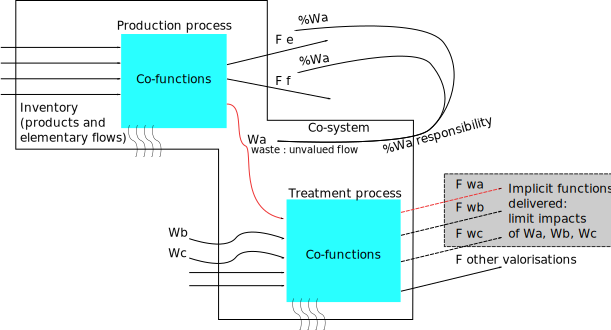
\includegraphics[width=\textwidth]{/home/rudy/Documents/rudy/01_These/11_production/01_COMMUNICATION/figures/co-treatment.pdf}
%}
% à remettre dans le .pdf_tex après modif : /home/rudy/Documents/rudy/01_These/11_production/01_COMMUNICATION/figures/
\caption{Une chaine de valeur introduisant l'allocation avec co-traitement et ses fonctions implicites.}
\label{fig:alloc_co-treatment}
\end{figure}
\figbox{
Dans la figure suivante (\ref{fig:alloc_co-treatment}), nous proposons d'associer la filière et le flux négativement apprécié.
%Often those process are modelled without their full functional spectrum.
%Heat or electricity production is observed.
%If any material flow can be used it is discussed (what substitution can be considered and so on).
%But implicit functions of treating the input flows are insufficiently documented.
%In the following figure, we propose to associate the treatment route to negatively valued flows.

L'allocation entre les flux co-traités peut être déterminée par leur part respective d'impacts calculés dans le cas d'une émission à la biosphère et suivant la matrice de jugement du décideur.
Plus le flux non traité aurait été jugé problématique, plus sa part d'inventaire est importante.
Ceci, pour le co-traitement, suit le même processus d'évaluation que pour les attributs des coproductions classiques.
%The allocation between co-treated flows can be elicited by their share of respective impacts \emph{if} they were released directly in nature \emph{and} following the decision maker judgement matrix. % ! précision sur le rejet à la biosphère sinon -> la poule et l'oeuf
%The more the flow would have been an environmental issue, the more its inventory is important.
%This is done following the same process as evaluating attributes of co-products.

Ainsi l'inventaire alloué de la fonction délivrée $F_e$ est l'allocation des coproductions avec $F_f$ et sa part de l'inventaire pour sa part respective de fonction $F_{Wa}$.
La part $W_a$ décharge l'excédent au dessus des 100~\% de l'inventaire initial et ajoute son propre inventaire pour $F_{Wa}$.
%So the allocated inventory of delivered function $F_e$ is the allocation of the co-production with $F_f$ and its share of inventory for its respective share of function $F_{Wa}$.
%$W_a$'s share unburden the excess above 100~\% of the inventory and its own inventory for $F_{Wa}$ adds up
}

%\begin{figure}
%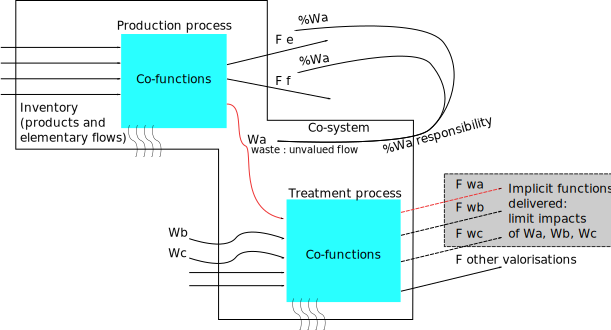
\psfig{file=/home/rudy/Documents/rudy/01_These/11_production/01_COMMUNICATION/figures/co-treatment.pdf_tex,width=4.5in}
%\caption{A process chain schema to introduce allocation with co-treatment case.}
%\label{aba:alloc_co-treatment}
%\end{figure}

%?
%This would remain simple if the value systems were stable and consistent.
%But they are nothing of the sort.
%The range of derivation techniques do not gives a unique solution.
%
%? DVP outranking ?
%So we propose to treat selection of alternative scenario after the LCIA results trough the highest frequency of preference.

%\subsubsection{A monte-carlo based preference}
%
%Based on multiple value judgement matrix, we could repeat LCA's calculation and depict the frequency at which the alternative is prefered.
%To reduce the number of calculation loops, the inconsistent terms on their respective side of the matrix's diagonal would be selected on the difference of their inverse.
%This way we could calculate the results on strongest value contradiction.
%Thus saving calculation times, we could more quickly see the preference divergence.
%On top of inconsistencies from human judgements, a sensitivity analysis shall be conducted in order to pinpoint the strongest link between the value matrix and the modeled system.

%\colorbox{yellow}{TRANSLATION INCOMMING}
Cette proposition, pour être employée, requière que les propriétés et destinations des flux et fonctions soient étudiées.
Ceci appelle au lien entre \gls{ACV} et \gls{MFA}, un courant déjà en marche dans la discipline~\cite{pauliuk_lifting_2015}.
\emph{Mais plus que la traçabilité des produits et substance (MFA actuel), il s'agit ici de réaliser la traçabilité des propriétés, de la façon dont elles sont délivrées et appréciées.}
\exbox{
Par exemple, la masse est habituellement employée pour révélée la quantité de matière, mais elle n'est pas nécessairement la propriété faisant l'intérêt de l'objet.

Du point de vue de la conception industrielle, nos besoins portent plus généralement sur des \emph{surfaces fonctionnelles}.
Remplir de matière pour supporter les contraintes entre ces surfaces nécessite un volume.
Le matériau choisi, répondant adéquatement aux contraintes et porteur d'une certaine densité \emph{implique} donc une masse.
%This proposal, to be used, requests that use properties and destinations be studied.
%This calls for linking LCA to MFA, actually "Lifting Industrial Ecology Modeling to a New Level of Quality and Transparency"~\cite{pauliuk_lifting_2015}.
%But not only tracking products and substances (MFA), doing so means tracking the use properties and how they are delivered and valued.
%For instance, mass is usually used to reveal an amount of material, but it is not necessarily the property that is of interest.
%From design and engineering perspective I'd say we usually need surfaces (functional ones).
%Filling material to support strains between these functional surfaces is the needed volume.
%The material that reply adequately to constraints bearing a density properties comes with a mass.

En nutrition, (pour la flore comme la faune), ce qui est recherché n'est pas une masse de nourriture mais une quantité d'énergie (kcal sur nos emballages), la présence de certains acides aminés et autres.
Ainsi dans ces cas la masse n'est qu'une conséquence de la recherche d'autres propriétés.
%In nutrition (human, animal or plant) what is sought is not the general mass of food, but to provide an amount in energy (kcal), and content in amino acids and else.
%So in those two case, mass would simply be a consequence not a requirement.

Plus occasionnellement la masse fournie une inertie et permet par gravité de garder des choses en place.
Ou encore pour un usage marketing, la masse est employée avec un discours 'lourd=robuste'.
%More occasionally mass is used to provide inertia or kip things in place or as marketing in "heavy = robust" discourses.

Comme il s'agit d'une façon pratique de gérer des quantités de produits délivrant d'autres propriétés appréciées, nous avons tendance à réduire notre intérêt et nos recherches à la seule masse des produits.
%As it is an easy way to handle the amounts of the products that deliver all these properties of interest, we tend to reduce requests and research to a mass of a specific product.
Il nous faut développer le spectre de propriétés de nos investigations.
%We have to develop the property spectrum of our investigations.
}
\subsection{L'intention et la destination}
Le système d'allocation multicritère diffère de la solution existante car il permet la réalisation d'une partition sur la base de co-fonctionnalités totalement hétérogènes.
De plus elle porte dans son principe l'expression explicite des jugements de valeur nécessaires à la distinction entre observations factuelles -- domaine objectif -- et le jugement moral -- domaine subjectif.
%Our multi-criteria system in opposition to prior methods enabled heterogeneous co-products to support partitioning with explicit priorities on values.
Cette nouvelle méthode ouvre des perspectives de valeurs en rendant la distinction initiale entre primaire et secondaire inutile.
Cela permet le traitement en plaine lumière de deux autres enjeux interconnectés, l'intention et la destination.
%However two linked points need digging in the matter of allocation --
%intention and actual use.

\textsc{Weidema} relève une distinction faite la génération précédente par Huppes (1992)~\cite{weidema_avoiding_2000}, une cause probable de problèmes dans la norme ISO et les guides attentant.
Il déclare que
\blockcquote[traduction]{weidema_has_2014}{la hiérarchie de l'allocation pourrait être significativement simplifiée si une séparation était faite entre les cas de coproduction avec une relation variable entre les coproduits et les situations de productions jointes par des relations fixes.}

Si nous écartons le cas ou des relations indépendantes peuvent être établie entre des coproductions et les paramètres d'entrées (c'est à dire une subdivision déguisée), que reste-t-il de l'argument~?~:
Le fait qu'une volonté puisse modifier les `points de fonctionnement' du système.

%\footnote{
%\blockcquote{weidema_avoiding_2000}{An important distinction must be made between joint production, in which the relative output volume of the co-products is fixed, and combined production, with independently variable output volumes (Huppes 1992)}
%}.

%L'argument est que le co-produit utilisé dans le système étudié sera consommé depuis ce procédés à relation variable.
%L'accroissement de quantité produite du fait de la variabilité serait donc équilibré avec ladite consommation\footnote{
%\blockcquote{weidema_avoiding_2000}{For the latter type of production, allocation can be avoided simply by modeling directly the consequences of a change in the output of the co-product of interest (that which is used in the product system under study) without change in the output of the other co-products. This situation is dealt with in step 1 of the procedure.}
%}
%Nous relevons toutefois que si la relation est variable ne pas changer le volume de production des autres coproduits de ce procédé équivaut à un accroissement de l'activité (procédé).
%C'est avec l'hypothèse d'élasticité des prix nulle, une hypothèse additionnelle... où finalement la critique de l'\textit{arbitraire} partition (qui en fait devrait dire subjectif) pourrait se voir opposer l'arbitraire projection économique.

La question que nous soulevons est la suivante~: En quoi le fait qu'une personne puisse interagir avec les parts des différentes productions modifie les propriétés d'usage ou d'échange des flux produits~?
%The intent and application case in allocation.
%\textsc{Weidema} points out a cause of trouble in ISO and guidelines.
%\blockcquote{weidema_has_2014}{The allocation hierarchy could be significantly simplified if a separate description was made for situations of combined production with variable relationships between the coproducts (...) and situations of joint production with fixed relationships}.
%The question we rise is: would the fact that one can manage shares of the flows modify the attributes of co-products?
Un flux désirés plus fortement (c'est à dire plus haut dans les rangs de préférences des co-fonctionnalités générés) se verrait produit en plus grandes quantités \emph{si} cela est possible.
%In our opinion a more desired flow would simply be of higher rank in the preference system and so be produced to more important quantities than its co-products \emph{if} possible.
Le fait qu'une personne n'ait pas voulu produire une chose, n'ôte pas à cette chose les attributs qu'elle recèle et la valeur potentielle qu'une tiers personne puisse attribuer à ses caractéristiques.
Gare toutefois aux confusions entre les propriétés de l'objet et des flux d'échanges de l'objet.
C'est là toute l'importance de traiter le problème dans sa complexité.
Un produit utile mais très largement répandu n'aura pas les même propriétés d'échange, propriété \textbf{extrinsèque}.

Mais ne nous arrêtons pas trop tôt en explication~: les circonstances déterminant les propriétés extrinsèques de l'objet ne sont (hors monopole ou oligopole très concentré) pas déterminée par un seul acteur en capacité d'influer sur elle.
C'est donc l'état \emph{des} destinations possibles qui les détermine.
%The fact that someone don't want to produce something does not suppress
%%the attributes it bears and 
%the potential values someone else may consider in them.

Ceci règle donc la question de l'intention, mais pas encore celle de la destination.
Le second point relève à la fois de savoir si le flux produit est effectivement employé et où, mais également \emph{pourquoi}, la \emph{destination} (dans toutes ses dimensions).

La question de la finalité de l'objet doit-elle intervenir dans la détermination de ce que nous jugeons nécessaire à son obtention~?
Doit-on considérer l'acier des fusils comme plus impactant que celui du matériel médical~?
Quelle distinction doit être faite entre un produit intermédiaire et un produit final~?
Que faire des produits finaux eux-mêmes multifonctionnels, comme par exemple la machine de calcul utilisée à la fois en "commerce haute fréquence" et pour la bio-informatique~?
%A second concern is what shall be made of useful but not used productions?

C'est ici que l'analyse des flux de produits, Material Flow Analysis (MFA), est la plus essentielle.
Si la destination d'un produit peut être suivie et documentée, alors déterminer qu'un produit apporte (ou non) tel \emph{service} est envisageable.
Dire qu'à l’accroissement ou à la réduction du flux disponible, telle application sera le "véritable procédé joint"~\cite{european_commission_ilcd_2010}, c'est encore traiter de cette question.
%This is where Material Flow Analysis (MFA) is most required.
%A use factor should go along each flow, either as a particular attribute or a value trigger.
%Unvalued and un-used flows would remain burdens when used, valued flows would allow partitioning of linked inventories.
\keybox{
La question de la destination future comme de ses seuils d'activation ou désactivation est en fait la part conséquentielle présente dans \textbf{chaque} étude d'\gls{ACV}.
Résoudre la multifonctionnalité nécessite de réaliser ce pan de l'étude.}

%Celle des destinations passées reste nécessaire pour l'angle attributionnel.
Notre modèle pour son emploi \emph{complet} requière donc que les propriétés d'usages \textbf{et} leurs destinations soient étudiées.
\emph{Ceci appelle à la liaison entre ACV et MFA.}
C'est un appel à \blockcquote{pauliuk_lifting_2015}{élever la modélisation de l'écologie industrielle à un nouveau niveau de qualité et de transparence}.
`Pas de transparence des chaînes de valeurs' égal `pas d'évaluation consistante de la soutenabilité'.
%This proposal, to be used, requests that use properties and destinations be studied.
%This calls for linking LCA to MFA, actually "Lifting Industrial Ecology Modeling to a New Level of Quality and Transparency"~\cite{pauliuk_lifting_2015}.
%But not only tracking products and substances (MFA), doing so means tracking the use properties and how they are delivered and valued.
%For instance, mass is usually used to reveal an amount of material, but it is not necessarily the property that is of interest.
%From design and engineering perspective I'd say we usually need surfaces (functional ones).
%Filling material to support strains between these functional surfaces is the needed volume.
%The material that reply adequately to constraints bearing a density properties comes with a mass.
%In nutrition (human, animal or plant) what is sought is not the general mass of food, but to provide an amount in energy (kcal), and content in amino acids and else.
%So in those two case, mass would simply be a consequence not a requirement.
%More occasionally mass is used to provide inertia or kip things in place or as marketing in "heavy = robust" discourses.
%As it is an easy way to handle the amounts of the products that deliver all these properties of interest, we tend to reduce requests and research to a mass of a specific product.
%We have to develop the property spectrum of our investigations.
%And the valuation of properties shall remain a reflect of the decision maker's orientations.

%This proposal doesn't solve all allocation issues.
%But it enable engaging in new development paths.
%\vspace{-0.3cm}
\section{Multifonctionnalité traitée par expansion}

Considérons maintenant l'option défendue par \citeauthor{weidema_avoiding_2010} d'éviter l'allocation~\cite{weidema_avoiding_2010,weidema_avoiding_2000}. \textbf{Est-il possible d'éviter l'allocation~?}
Il n'est pas ici question de substitution ni même de mise à l'échelle.
Nous avons traité dans la description des méthodes de traitement de l'allocation de ces nuances.
Ici, une \textbf{pure expansion} de l'unité fonctionnelle aux co-fonctions remplies par le système observé doit être réalisée.
C'est en somme conserver pour l'inventaire la position de l'observation sans jugement.

Le résultat est donc la confrontation d'ensembles de fonctionnalités délivrées et d'impacts associés.
Il s'agit donc au stade de l'interprétation de définir la préférence du décideur envers ces ensembles.

Quelle(s) différence(s) y a-t-il entre l'application de la partition multicritère avec l'ensemble de la matrice de jugement du décideur à la constitution de l'inventaire et l'application du jugement après expansion ?


\begin{figure}
\centering
%\includegraphics{/home/rudy/Documents/rudy/01_These/11_production/01_COMMUNICATION/figures/alloc_value_integrated_20160226.pdf_tex}
\includegraphics[width=0.9\textwidth]{/home/rudy/Documents/rudy/01_These/11_production/01_COMMUNICATION/figures/partition_expansion.pdf}
% à remettre dans le .pdf_tex après modif : /home/rudy/Documents/rudy/01_These/11_production/01_COMMUNICATION/figures/
\caption{Partition et Expansion, quelles différences ?}
\label{fig:partition_expansion}
\end{figure}

%\begin{tcolorbox}[
%%					colframe=red!50!white,
%					width=\textwidth,
%%                  enhanced,
%%                  frame hidden,
%%                  interior hidden,
%                  boxsep=2pt,
%                  left=2pt,
%                  right=2pt,
%                  top=2pt,
%                  ]
\figbox{
La figure~\ref{fig:partition_expansion} représente par la symbolique de la balance le processus comparatif et le traitement de la multifonctionnalité d'abord par partition puis par expansion.
\keybox{
Il n'y a pas de véritablement 'meilleure' alternative mais uniquement des alternatives \emph{préférées}.
La question est donc de savoir quelle alternative est réellement préférée par le décideur.}
Il faut donc une unicité du jugement employé.
Les modes de traitement de la multifonctionnalité, consistant avec le caractère multi-critère de l'ACV, restent donc la partition multi-critère et l'expansion.
Dans le premier mode de traitement, le jugement du décideur est appliqué d'abord pour isoler l'unité fonctionnelle à la base de l'étude.
Puis il est appliqué une seconde fois pour déterminer l'alternative préférée parmi celle délivrant cette même unité fonctionnelle.
Ce premier type de traitement se limite donc à la confrontation de systèmes répondant à (au moins) une même fonction.
Dans le second mode de traitement, c'est l'ensemble des fonctions et impacts de chaque alternative qui est confronté aux autres.
\textbf{Il n'y a plus unicité de la fonction.}
Le jugement n'est appliqué qu'une fois sur la globalité de la confrontation.
Il sera donc remarqué que l'ensemble des jugements sur les fonctionnalités et impacts doit être disponible de façon globale et consistante.
}
%\end{tcolorbox}

%\colorbox{yellow}{ application numérique, reprendre fichier test allocation.ods et test electre.r}

%\subsection{Application comparée}
%
%Soit le cas (a) de la table~\ref{tab:allocation_partition_cas_dissociables}.
%Posons le cadre d'application~: un décideur s'interroge sur le choix entre le produit 1c et 2a.
%Ajoutons maintenant une donnée d'inventaire liée à un impact, disons~: 6~kg CO2 au produit 1 et 1~kg CO2 au produit 2.
%
%Puisque le système de valeurs intervenant ne porte plus uniquement sur le traitement de la multifonctionnalité mais la préférence entre deux modifications d'états alternatives (impacts), étendons le système de valeur.
%
%Le jugement sur les aires de protection est le suivant~:
%\begin{table}
%  \begin{center}
%  \caption{Matrice de comparaison par paires, visant les aires de protection, remplie à titre d'exemple. CI 0.0013 ; CR 0.0023}
%  
%  \begin{tabular}{| c|c |c |c |c|}
%  \hline
% & Éco-système & Vie humaine & Ressource & Priorité \\ 
% \hline
%Éco-système & 1     & 2     & 7     & 0,62 \\ 
%Vie humaine &  1/2 & 1     &  3 & 0,29 \\ 
%Ressource &  1/7 & 1/3     & 1     & 0,09 \\ 
%  \hline
%  \end{tabular}
%  \end{center}
%  \label{tab:3_attributs_impacts}
%  \end{table}
%Si l'on considère une architecture des valeurs où les dimensions monétaire, énergétique et massique porte sur la distribution des ressources, alors la hiérarchie définie à la table \ref{tab:exemple 3 attributs}, est incluse sous celle des aires de protection dans l'espace des ressources.
%Ceci nous donne le coefficient 0.09 en facteur sur ces valeurs.
%
%%Poursuivons notre application avec la position d'un acteur à but lucratif, pour lequel, les alternatives ont donc pour fonction principale d'être rémunératrice (conformément au système de valeur exprimé pour l'allocation).
%%Notons la contradiction sur les aires de protection...
%
%\subsubsection{Traitement par partition}
%La produit 1c est caractérisé par~:
%La fourniture de 13 EUR, 32 kg (mat non précisée) et l'émission de 6~kg~CO2 (en co-fonction avec le produit 2c), attribué à 37.1\% à 1c (soit 2.226~kg~CO2).
%La produit 2a est caractérisé par~:
%La fourniture de 8 EUR, 7 kWh (niveau énergétique non précisée) et l'émission de 1~kg~CO2 (en co-fonction avec le produit 2c), attribué à 60.7\% à 2a (soit 0.607~kg~CO2).
%
%Posons le surclassement suivant (cf section mcdm~\ref{mcdm}).
%
%\colorbox{yellow}{proposer un exemple avec promethee et un avec electre}
%
%\colorbox{yellow}{ré-installer les outils numérique ? (galère à la main)}
%
%\colorbox{red}{pas fini}
%%π(a,b)=∑j=1kwjPj(a,b)
%$ \pi(a,b)=\sum j=1kwjPj(a,b) $
% \begin{table}
%   \begin{center}
%   \caption{Surclassement entre 1c et 2a}
%   
%   \begin{tabular}{|c |c |c|}
%   \hline
%  critère & surclassement & puissance \\ 
%  \hline
% Éco-système &      & 2     \\ 
% \hline
%% Ressource &  1/7 & 1/3     \\ 
% Eur &  1c P 2a & 1     \\
% kWh &  2a P 1c & 1     \\
% kg & 1c P 2a  & 1      \\  
%   \hline
%   \end{tabular}
%   \end{center}
%   \label{tab:ex_surclassement}
%   \end{table}
%\subsubsection{Traitement par expansion}

%\section{La dimension politique}

\newpage
\section{Conclusion sur la multifonctionnalité}
\label{sec:Conclusion sur la multifonctionnalité}
\keybox{
La multifonctionnalité en ACV était un problème non encore résolu.
Plus qu'une formulation ambiguë des questions d'allocation~\cite{weidema_has_2014},
les limitations de l'ISO~14040 résident dans l'absence d'un élément central~: \emph{l'intégration globale, consistante et explicite, du jugement moral des parties-prenantes}, pour la résolution de cette question.
}
%xxxxxxxxxxxxxxxxxxxxxxxxxxx

Les caractéristiques à prendre en compte sont autant physiques qu'humaines.
Englober à la fois les perspectives physiques et socio-économiques, c'est tenter une réconciliation entre valeur d'usage et valeur d'échange, dans la continuité de travaux de longue date d'économistes antiques comme modernes~\cite{harribey_richesse_2013}.
C'est refuser d'accepter la seule lecture de la valeur imposée par la classe dominante.
C'est unir les dimensions de la réalité plutôt que de déterminer, ou imposer, une séparation et une hiérarchie entre elles comme certains le proposent~\cite{pelletier_rationales_2014}
\footnote{
\blockcquote[traduction]{pelletier_rationales_2014}{
Nous concluons que la hiérarchie de multifonctionnalité de l'ISO~14044 devrait explicitement faire une distinction entre les applications de modélisation des données attributionnelles et conséquentielles.[\ldots]

Nous suggérons que la norme ISO 14044 devrait également rendre explicite sa rationalisation pour \emph{privilégier les approches fondées sur les sciences naturelles} pour résoudre les problèmes de multifonctionnalité et de \emph{différencier plus clairement les approches fondées sur les sciences naturelles et  sur les sciences sociales.}
%We conclude that the ISO 14044 multifunctionality hierarchy should explicitly differentiate between attributional and consequential data modeling applications.
%(...) We suggest that ISO 14044 should also make explicit its rationale for \emph{privileging
%natural science-based approaches} to solving multifunctionality problems and to \emph{more clearly differentiate between natural science and social science-based approaches}
.}
}.

Parmi les dimensions objectives, nous relevons également l'importance pour les grandeurs extrinsèques d'une documentation riches des flux des produits et de leurs caractéristiques.
Le traitement par destination nécessaire notamment à la résolution des multifonctionnalité pour les semi-produits implique une documentation plus ouverte des processus industriels.
La tendance à la protection des secrets industriels pourrait bien priver les sociétés humaines de décisions rationnelles.
L'alternative à une donnée primaire issue des sites effectifs serait une reconstitution depuis la documentation des processus connus et employés dans les entreprises ouvertes (fonction publique ou établissement fonctionnant sur la base de l'open-source).

%Cette thématique, débutée semble-t-il avec \textsc{Aristotle}, est plus récemment traitée par \textsc{Harribeys}~\cite{harribey_richesse_2013}.
La recherche d'un traitement holistique est le rappel du caractère multidimensionnelle de la réalité et de l'\emph{incommensurabilité} de ces dimensions.
C'est reconnaître la multiplicité et la complexité, pour \emph{ne pas imposer de jugement unique}.

%Encompass both physical and socio-economic perspectives~\cite{pelletier_rationales_2014} is trying a reconciliation between use and exchange values.
%Question of what matters or matters most, 

%%This matter, discussed by \textsc{Aristotle}, is more recently browsed by \textsc{Harribeys}~\cite{harribey_richesse_2013}.
%Summing up this we would say, money has no monopoly on richness. %\footnote{"Richness" is used here to avoid a misleading use of "value" monetary value.}.
De surcroît, il est difficilement envisageable que notre société évolue vers une alternative \emph{soutenable}, pour elle toute entière, dans un saut à un système de valeur entièrement nouveau.
Il est en tout cas certain qu'une évolution vers une soutenabilité forte ne pourra se faire sur la base des deux principes~:
%\begin{enumerate}
(1) Les praticiens acévistes ne doivent pas mélanger les clefs d'allocation.
(2) L'allocation économique est le cas général.
%\end{enumerate}
%Furthermore, we can hardly imagine our society evolve in a jump to an alternative set of governing values.
%For sure it cannot be achieved while keeping the two statements: 1) LCA practitionners should not mix allocation keys 2) Economic allocation is the general case.

Alors que nous réalisons la sélection des \emph{valeurs} déterminantes du système, n'oublions pas~:
%\begin{itemize}
(i) les applications de l'information produite,
(ii) qui prend la décision
et (iii) qui en supportera les conséquences.
%\end{itemize}
L'ACV est utilisée pour \emph{Le développement des Produit} dans une économie globalisée ; en \emph{Marketing} et les produits discutés peuvent couvrir la planète ; en \emph{Planification Stratégique} et à l'\emph{élaboration des réglementations publiques}~\cite{european_commission_ilcd_2010}.\\
\textit{Ainsi, par ces évaluations sont écrites les orientations de ce qui va être,\\
et les conséquences qui seront supportées par tous, ainsi que ceux à naître.\\}
%While eliciting values, shall we not forget applications of the produced informations.
%\emph{Who} is the \emph{decision maker} and \emph{who will support the consequences}.
%\cite[Framework for life cycle assessment (from ISO 14040:2006; modified)]{european_commission_ilcd_2010}.
%LCA is used for ``\emph{Product development and improvement}'' in a global economy.
%It is used in ``\emph{Marketing}'' and the discussed product can cover the globe.
%It is used for ``\emph{Strategic planning}'' and ``\emph{Public policy making}''.
%So orientations of what will be tomorrow are written there and \emph{the consequences will be borne by everyone even those yet to be born}.
Conséquemment allons un pas plus loin dans le sens de la déclaration de \textsc{Mathe}~\cite{mathe_integrating_2014}.
Intégrer les parties prenantes n'est pas uniquement \emph{intéressant}, c'est une \emph{nécessité}.
%Consequently we propose going a step further with respect to \textsc{Mathe}'s statement~\cite{mathe_integrating_2014}.
%Integrating stakeholders participation is not only \emph{of interest}, it is \emph{necessary}. % to avoid LCA's failure.
Il est donc apparu crucial de concevoir une méthodologie permettant une modification interactive et progressive du système de valeurs à la base de nos décisions. 
%So we devised a consistent method allowing for a progressive and interactive modification of the value balance.

%xxxxxxxxxxxxxxx


Nous avons exposé l'usage du modèle multicritère produit pour l'allocation et ses résultats sur des sorties (flux sortants) \emph{hétérogènes}.
Nous avons souligné l'importance de développer les priorités sur l'\emph{ensemble} des valeurs manipulées en ACV \emph{avec} les parties-prenantes.
%We exposed its use for allocation and its results on heterogeneous outputs and stressed out the need to develop priorities on \emph{all} values handled in LCA \emph{with} stakeholders. 
\keybox{
Comme des attributs incommensurables\footnote{Sans commune mesure.} sont en jeu, \emph{nous ne pouvons pas nous passer de l'expression d'opinions}.
La capacité de l'ACV à se développer en tant que science sera directement liée à notre capacité à dissocier observations, opinions et leur traitement conjoint.
Les façons dont nous organiserons la détermination des jugements de valeurs pour nos processus de décisions seront les miroirs de nos cultures.}
%As incommensurable attributes are at stake, \emph{we can not bypass the expression of opinions.} % if we are to include these attributes}.
%The capacity for LCA's field to develop as a science will be the direct result of our ability to dissociate observations,
%% and its data, the needed 
% opinions and the processing of both.
%The way we will organize this values elicitation in our decision process will be the mirror of our societies cultural portraits.

Il convient donc de modifier en conséquence la norme de l'ACV.
La modification est représentée au~\ref{sec:Un nouveau standard}.
L'étape de déclaration de valeurs, pour des raisons de consistance, devrait viser à la fois les attributs des flux pour le traitement de la multifonctionnalité et les impacts pour l'interprétation.
%Allocation in LCA is an issue.
%But more than ambiguous phrasing of multi-functionality treatment~\cite{weidema_has_2014}, %in my opinion
%ISO~14040
%%serie
%'s limitation lies in its lack of a central key element: \emph{explicit stakeholders value judgements integration}.
%The value declaration step should target both attributes for allocation and impacts for interpretation %.
%It should
Cette étape devrait être traitée avant même la définition du but de l'étude~\cite{patard_life_2015}.
%and
%it should be treated before defining the goal of the study~\cite{patard_life_2015}.
Elle serait une étape indépendante de l'ACV, bien que fournissant une part d'information cruciale à sa réalisation.
Réaliser ce 'découpage' permettrait un processus de revue effectif des ACV.
L'application effective du jugement du décideur pourrait être contrôlée.
Les bases de données contiendrait alors les descriptions des systèmes techniques, environnementaux et sociaux.
Il serait donc possible de fournir ce qui est requis par certains auteurs \blockcquote{majeau-bettez_unified_2014}{la dissociation de l'observation (inventaire) de la modélisation}.
%It is an independent step of LCA, even though providing necessary information for it.
%Doing so would allow effective reviewing process %.
%and
%%It would 
%enable LCA to effectively reflect the judgement of the decision maker(s).
% would be independent of the judgement.
%Databases would then be systems descriptions for social, environmental or technical information.
%It would then become possible to deliver what is required by some authors\blockcquote{majeau-bettez_unified_2014}{to dissociate the observation (inventory) from the modelling}.

Nous allons donc dans la partie suivante observer comment produire cette unicité du jugement.